% 'draft' mode can be used to speed up compilation
\documentclass[twoside,final]{hcmut-report}
\usepackage{codespace}

% Draft watermark
% https://github.com/callegar/LaTeX-draftwatermark

% Encodings
\usepackage{gensymb,textcomp}

% Better tables
% Wide tables go to https://tex.stackexchange.com/q/332902
\usepackage{array,longtable,multicol,multirow,siunitx,tabularx}

% Better enum
\usepackage{enumitem}

% Graphics
\usepackage{caption,float}

% Add options for figures, like max width, framing, etc.
\usepackage[export]{adjustbox}

% References
% Use \Cref{} instead of \ref{}
\usepackage[nameinlink]{cleveref}
\usepackage[version=4]{mhchem}

% Additional packages can be added here as needed

% Sub-preambles
% https://github.com/MartinScharrer/standalone

% Configurations
\coursename{ES-243-CC01 - Earth Science}
\reporttype{MUSEUM REPORT}
\title{MUSEUM REPORT}
\advisor{& MSc. Dong Uyen Thanh &}
\stuname{%
  & Nguyen Le Thanh Hao & 1952242 \\
  & Pham Gia Bao & 2151052 \\
  & Nguyen Bao Duy & 2152042 \\
  & Vo Minh Nhat & 2151240 \\
}

% Allow page breaks inside align* environment
%\allowdisplaybreaks{}

% Makes a lot of things blue, avoid at all costs
%\everymath{\color{blue}}

% Set depth of numbering for counters
\AtBeginDocument{\counterwithin{lstlisting}{section}}

% Rename some sections
%\AtBeginDocument{\renewcommand*{\contentsname}{Contents}}
%\AtBeginDocument{\renewcommand*{\refname}{References}}
%\AtBeginDocument{\renewcommand*{\bibname}{References}}

% Custom commands
%\newcommand*\mean[1]{\bar{#1}}

\begin{document}
\coverpage%

% Set table of contents depth to only show sections (not subsections)
\setcounter{tocdepth}{1}

\tableofcontents
\listoffigures
\listoftables
\lstlistoflistings{}

\clearpage

% Import acknowledgement
\section*{ACKNOWLEDGEMENT}
\addcontentsline{toc}{section}{ACKNOWLEDGEMENT}

We would like to express our sincere gratitude to MSc. Dong Uyen Thanh for her guidance and support during our study at the Ho Chi Minh City Geological Museum. Through her lectures and explanations, we gained not only theoretical knowledge but also practical insights into rocks, minerals, and the broader concepts of geology. The detailed stories and real-life examples she shared helped us better understand the subject and connect classroom knowledge with real-world applications.

The experience at the museum has provided us with valuable resources for future projects and strengthened our awareness of the Earth, encouraging us to care for and protect it. In this report, we have done our best to apply the lessons and knowledge received from Ms. Thanh, along with additional reference materials. Despite our efforts, some minor errors in grammar or understanding may remain.

Once again, we sincerely thank MSc. Dong Uyen Thanh for giving us the opportunity to learn through such a meaningful and practical experience.

\clearpage

% Import chapters
\section{INTRODUCTION}
\label{sec:introduction}

In the distant past, meteorites of enormous size flew through the Earth's atmosphere and crashed into our planet; these collisions vaporized mineral fragments from the ground and sent them into the sky. The molten minerals floated in the air like sparkling raindrops, each one traveling thousands of kilometers before falling back to the ground. Even further back, the collision of two hot celestial bodies caused the formation of the Earth and the Moon as we know them today, with the Earth carrying a multitude of minerals within it. After millions of years buried under layers of rock, these shiny mineral fragments occasionally rose to the surface to tell of the vastness of the Earth and the immensity of time.

Geology is the study and combination of knowledge about how rocks form over thousands of years, how fascinating gemstones can be created under pressure and temperature, how minerals are formed, and also about fossils and geological heritage. The Earth was formed about 4.6 billion years ago, so there must be beautiful formations of rare rocks, or even gemstones hidden somewhere within the Earth. Therefore, learning about the theory of rocks and minerals through books will only get us halfway through the actual knowledge of Earth geology. As President Ho Chi Minh taught us: "Learning must go hand in hand with practice. It is useless to study without practice; if you don't learn, you won't be fluent."

Therefore, we went on a trip to visit the Ho Chi Minh City Geological Museum as part of a learning activity, to practice observing and understanding the geological history of Vietnam, with the formation of rocks, ores, minerals, and even gemstones.

\subsection{Museum Overview and Visit Objectives}
\label{subsec:museum-overview}

\begin{figure}[H]
  \centering
  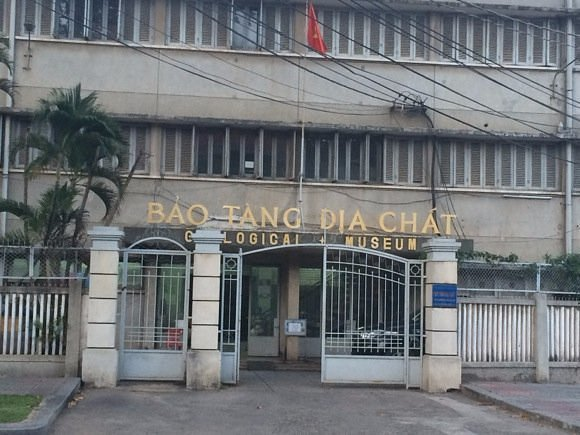
\includegraphics[width=0.8\textwidth]{graphics/figure_01.jpg}
  \caption{Ho Chi Minh City Geological Museum}
  \label{fig:museum}
\end{figure}

The visit to the Ho Chi Minh City Geological Museum provided us with a valuable chance to connect the theories we learned in class with real-world examples. While books and lectures give us the foundation of geological knowledge, nothing compares to directly observing the specimens that reflect millions, even billions, of years of Earth's history. At the museum, we could see how rocks, ores, minerals, and gemstones are preserved and displayed, each telling a story about the planet's formation and transformation over time.

This experience not only strengthened our understanding of the processes that shape the Earth but also gave us a clearer view of Vietnam's own geological heritage. By exploring these collections, we were able to develop a deeper appreciation of geology as both a science and a record of natural history. More importantly, the museum visit allowed us to practice critical observation, linking theory with practice, and to better prepare for future studies and projects related to Earth sciences.

\subsection{Museum History and Significance}
\label{subsec:museum-history}

The Geological Museum has a long history closely tied to the development of geological research in Vietnam since the colonial period. In 1898, the French colonial government established the Indochina Geological Service (Service Géologique de l'Indochine) and initiated the construction of a museum dedicated to geological research and education. By 1914, the museum's first building was completed in Hanoi. After the Geneva Agreement in 1954, part of the collection was moved to Saigon, where it was initially displayed in a temporary villa before being relocated to its current building in 1973. Following national reunification, the museum was managed by the Southern Geological Mapping Federation and continued to expand within the national geological system.

In 2001, it became one of the first museums in Vietnam to be recognized by the International Council of Museums (ICOM). In 2003, the Geological Museum system was restructured under the Department of Geology and Minerals, and in 2008, the Ho Chi Minh City branch was officially integrated as the southern division. Today, the Geological Museum stands as Vietnam's national geological museum, operating under the Department of Geology and Minerals of the Ministry of Natural Resources and Environment.

The museum currently holds about 13,000 precious geological specimens, of which about 3,000 are on permanent display. Including geological drill cores and archived samples, the total number of specimens here is more than 20,000. The highlight on the ground floor (General Geology) is the 1:500,000 scale geological map of Vietnam completed in 1988. This large map shows the geological structure of the entire territory of Vietnam clearly annotated, very useful for visitors to learn about the diversity of resources and stratigraphy.

This report will illustrate our visit to the Ho Chi Minh City Geological Museum, particularly focusing on Floor 1 and Floor 2. The first floor of the Museum will briefly introduce the geological evolution of Vietnam with the geological processes. On the second floor, we will demonstrate the fuel, metallic and non-metallic minerals, gemstones, mineral water and the concept of geological heritage. Throughout this report, we will organize the geological knowledge and our own experience to make this report more informative and easier to comprehend.
\section{GENERAL GEOLOGY (The 1st Floor Room)}
\label{chap:general-geology}

\section{Geological evolution}
\label{sec:geological-evolution}

The Earth has experienced a vast and dynamic history of about 4 billion years. This journey is divided into major geological eons and eras, each defined by important events such as the formation of the crust, shifts in the atmosphere, the rise of life, and tectonic movements. These processes become clearer when explored alongside physical specimens and visual displays, such as those presented at the Ho Chi Minh City Geological Museum.

\subsection{Precambrian: 4 billion to 570 million years ago (~600 million years)}
\label{subsec:precambrian}

\subsubsection{Archean Eon (4.0–2.6 billion years ago)}
\label{subsubsec:archean}

It is one of the earliest chapters in Earth's history, when the crust stabilized, continents and oceans first formed, and simple life such as stromatolite-building cyanobacteria appeared, slowly altering the planet's atmosphere.

In Vietnam, Archean rocks are found in the Kon Tum geoblock, mainly within the Kan Nack Group. These 3,000-meter-thick metamorphic rocks show complex changes, from granulite facies to amphibolite and greenschist facies, revealing the intense geological processes that shaped the ancient Earth.

\begin{figure}[H]
  \centering
  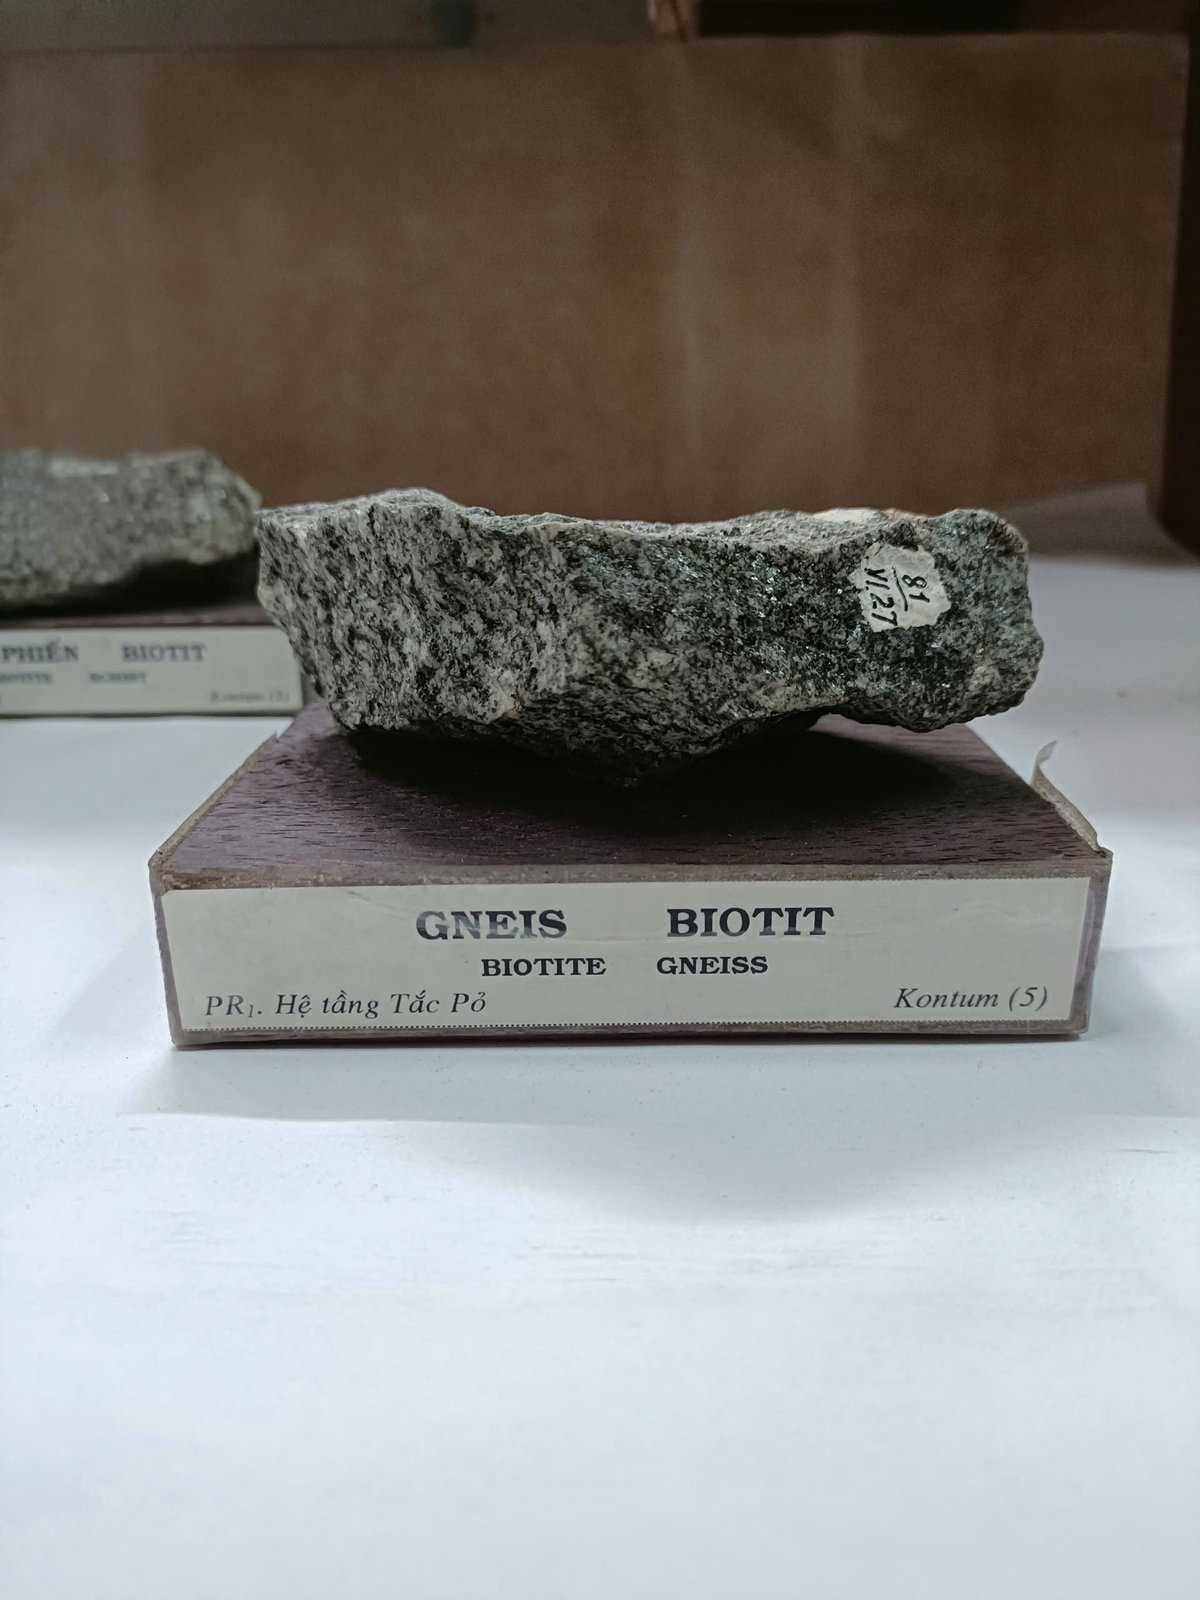
\includegraphics[max width=0.8\linewidth]{graphics/figure_02.jpg}
  \caption{Sample of rock in Archean Eon}
  \label{fig:archean-rock}
\end{figure}

\subsubsection{Proterozoic Eon (2.6 billion to 570 million years ago)}
\label{subsubsec:proterozoic}

It saw the Great Oxidation Event, global ice ages called "Snowball Earth," and the rise of the first multicellular life, including the Ediacaran biota. These changes prepared the planet for the Cambrian explosion of life.

In Vietnam, rocks from the Proterozoic are found in areas like Red River, Fansipan, Chay River, Ma River, Phu Hoat, and Kon Tum. These include crystalline and metamorphic rocks as well as younger layers that lead into the Cambrian period. Some of these rocks contain fossils of tiny early life forms.

\begin{figure}[H]
  \centering
  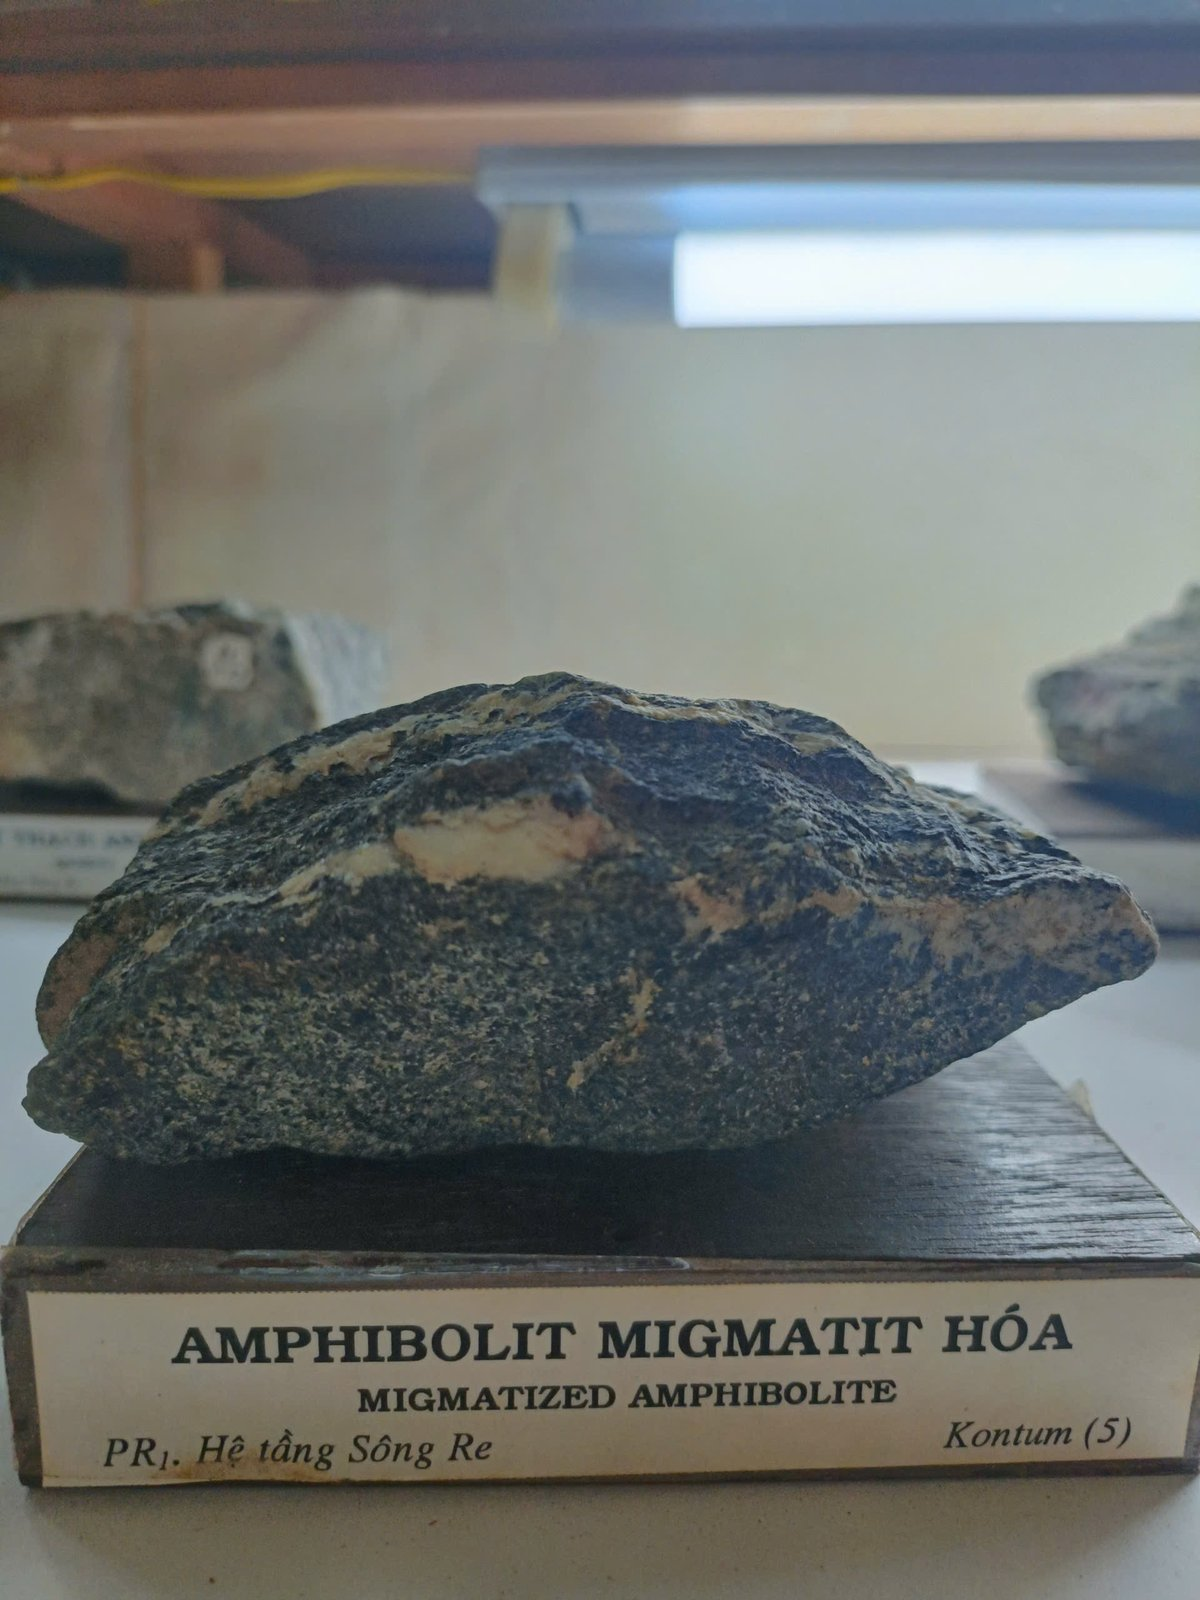
\includegraphics[max width=0.8\linewidth]{graphics/figure_03.jpg}
  \caption{Sample of rock in Proterozoic Eon}
  \label{fig:proterozoic-rock}
\end{figure}

\subsection{Paleozoic Era (541 – 252 million years ago)}
\label{subsec:paleozoic}

This era began with the Cambrian Explosion, a massive diversification of marine life. It is divided into six periods: Cambrian, Ordovician, Silurian, Devonian, Carboniferous, and Permian. During this time, ocean life expanded rapidly with animals like trilobites, corals, crinoids, brachiopods, graptolites, and cephalopods. Later, plants and amphibians colonized land. The era ended with the Permian-Triassic extinction, the largest known mass extinction, wiping out over 90\% of marine species.

In Vietnam, marine sedimentary rocks with abundant fossils (e.g., corals, brachiopods, trilobites) are found in Northeast Vietnam, such as in Cao Bang and Ha Long Bay. The Truong Son (Annamite) Range began forming due to Caledonian and Hercynian orogenies. Many rocks from the Paleozoic Era can still be found today in regions like North Vietnam, Northwest Vietnam, Northeast Vietnam, and Central Vietnam, where the rocks are made of limestone and other sediments that contain fossils of trilobites, brachiopods, and corals.

At the museum, fossils of corals, mollusks, and petrified wood from areas like Truong Sa (Spratly Islands) and northern Vietnam are exhibited. Geological maps display Paleozoic strata across northern and central Vietnam.

\begin{figure}[H]
  \centering
  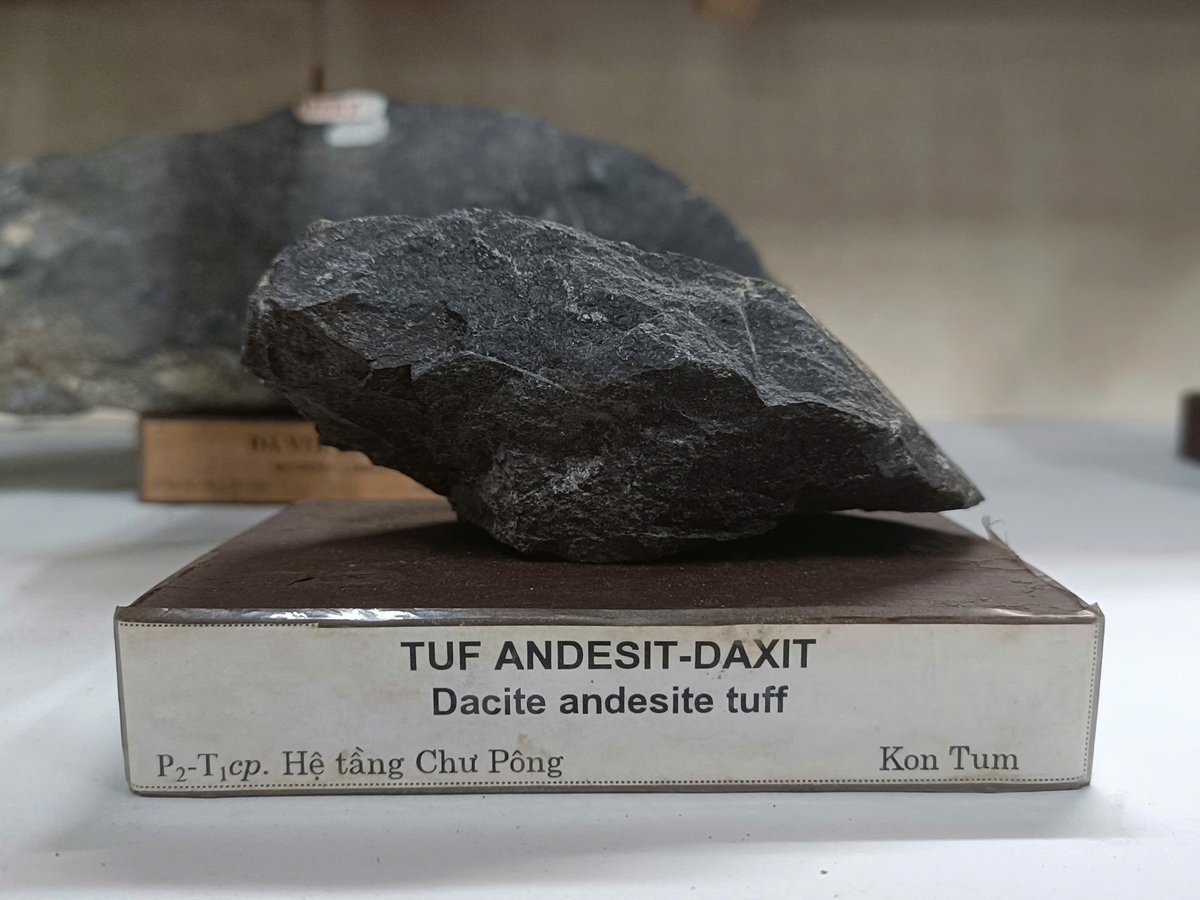
\includegraphics[max width=0.8\linewidth]{graphics/figure_04.jpg}
  \caption{Sample of rock in Paleozoic Era}
  \label{fig:paleozoic-rock}
\end{figure}

\subsection{Mesozoic Era (252 – 66 million years ago)}
\label{subsec:mesozoic}

Known as the "Age of Dinosaurs," the Mesozoic saw the rise of reptiles, the breakup of Pangaea, and generally warm climates. It is divided into three periods: Triassic, Jurassic, and Cretaceous. This era is famous as the "Age of Reptiles," when dinosaurs, ammonites, and many other creatures lived, along with early plants and marine animals like bivalves and brachiopods. The era ended with the Cretaceous–Paleogene (K–Pg) extinction caused by the Chicxulub impact and Deccan volcanism.

In Vietnam, the Indosinian Orogeny uplifted the Truong Son Range and created sedimentary basins. Volcanic and sedimentary activity occurred in areas like Kon Tum, Son La, and Thanh Hoa. Fossil evidence of dinosaurs and ancient flora has been found in some localities. Mesozoic rocks are found in places such as An Chau, Da River, Hien River, and Southwest. Triassic rocks here contain fossils of ammonites, gastropods, plants, and bivalves. Later, during the Jurassic and Cretaceous, red continental rocks and coal-bearing formations appeared, especially in the North, while volcanic rocks developed in areas like Tam Lang and Tu Le. These layers preserve fossils that show how both land and sea environments changed during this era.

At the museum, basalt and volcanic sediment from this era are displayed in the "Magmatism" section. Fossils and stratigraphic profiles reflect the Mesozoic biosphere and tectonic events.

\begin{figure}[H]
  \centering
  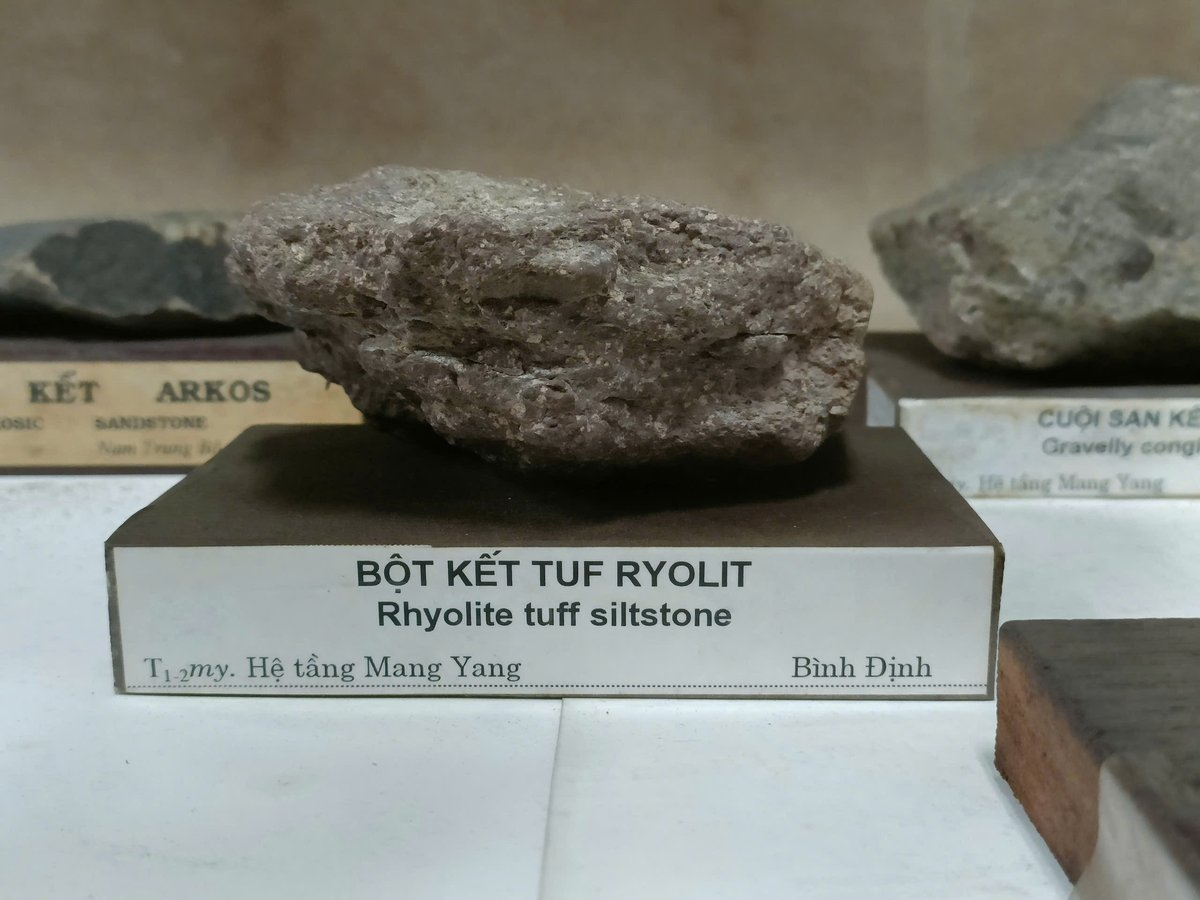
\includegraphics[max width=0.8\linewidth]{graphics/figure_05.jpg}
  \caption{Sample of rock in Mesozoic Era}
  \label{fig:mesozoic-rock}
\end{figure}

\subsection{Cenozoic Era (66 million years ago to present)}
\label{subsec:cenozoic}

This era features the evolution and dominance of mammals, birds, and eventually humans. Tectonic faulting, glaciations, and sedimentation shaped modern landforms and ecosystems. It is divided into three periods: Paleogene (66–23 million years ago), Neogene (23–2.6 million years ago), and the Quaternary (2.6 million years ago to today). This era is marked by great diversification of life, with many plants, mollusks, diatoms, ostracods, foraminifers, and vertebrates flourishing.

In Vietnam, major faults like the Red River and Song Ca faults influenced the formation of the Cuu Long (Mekong) and Red River basins, rich in oil and gas. The Quaternary Period (~2.58 Ma - present) witnessed alternating glaciations and interglacials, forming the Mekong and Red River deltas through alluvial deposition. Cenozoic rocks are found in regions such as Northwest (Pu Tra, Nam Bay), South Central Coast, and coastal basins. Paleogene rocks are rare, but Neogene sediments are widespread, often containing coal, kaolin, bentonite, and diatomite. These layers also include volcanic rocks, lagoon and delta deposits, and shallow marine formations, preserving fossils that show the rich environments of Vietnam during this era.

At the museum, core samples of crude oil from the Cuu Long basin (collected in the 1980s) are on display. Sediment cores and alluvial rock samples reflect recent geological processes, showcased in the "Fuel Group" and sedimentary sections.

\begin{figure}[H]
  \centering
  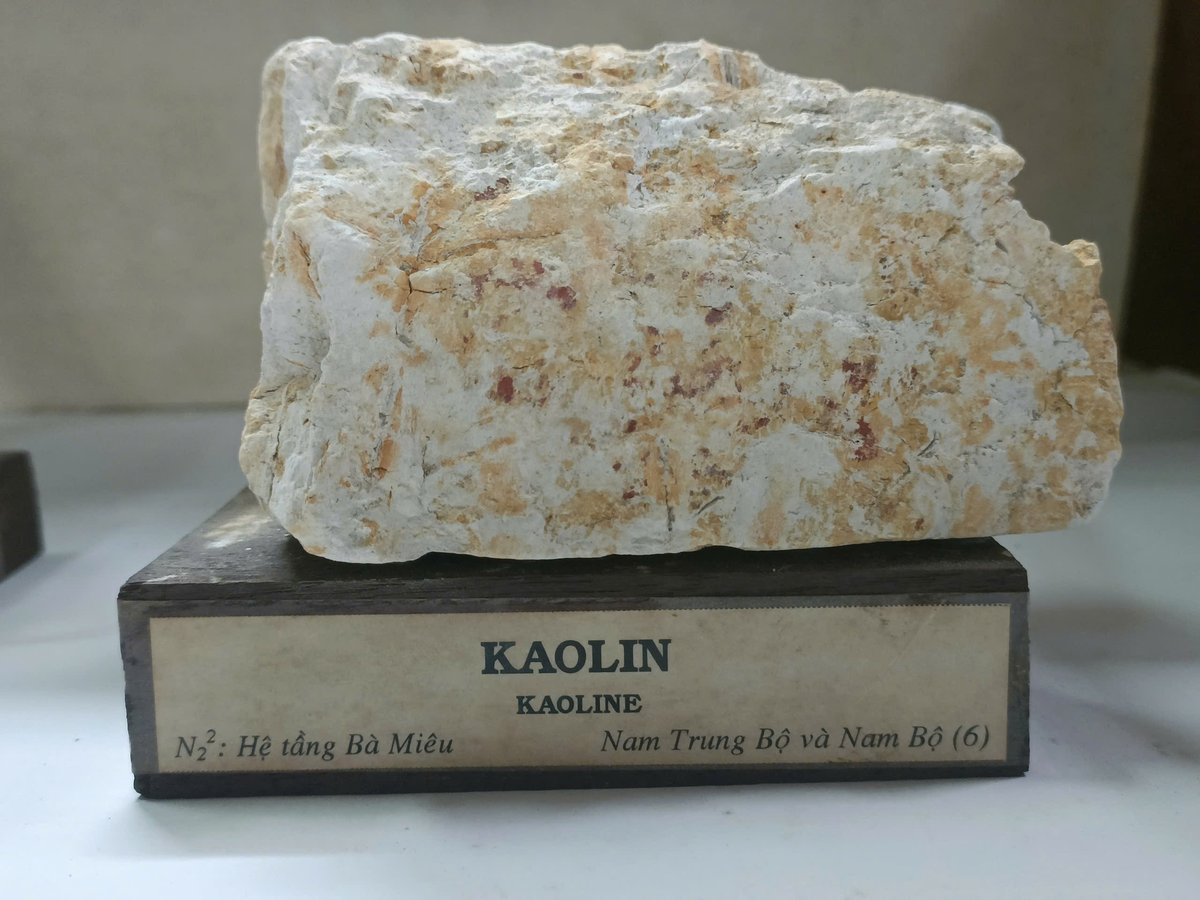
\includegraphics[max width=0.8\linewidth]{graphics/figure_06.jpg}
  \caption{Sample of rock in Cenozoic Era}
  \label{fig:cenozoic-rock}
\end{figure}

\section{Geological Process}
\label{sec:geological-process}

Geological processes are natural forces that continuously shape and alter both the Earth's surface and its interior. At the Ho Chi Minh City Geological Museum, visitors were introduced to six key geological processes through rock samples, models, and diagrams. These processes—ranging from extraterrestrial impacts to deep-earth activity and surface transformations—drive the creation, modification, and recycling of Earth's materials. The museum's exhibits illustrated how each process contributes to the formation of various rocks and landforms, highlighting the dynamic and interconnected system of the geological cycle.

\subsection{Cosmic process}
\label{subsec:cosmic-process}

Although no meteorite samples were displayed during the visit, the cosmic process remains essential in Earth's geological history. It refers to extraterrestrial impacts, especially meteorites, which helped shape the early Earth. These collisions formed craters, altered surface rocks, and delivered elements like iron, nickel, and platinum - key components of Earth's crust and core. Despite the lack of exhibits, this process highlights the planet's cosmic origins and is widely studied through global meteorite discoveries.

\subsection{Tectonic process}
\label{subsec:tectonic-process}

Tectonic processes involve the movement of the Earth's lithospheric plates. These dynamic movements are responsible for geological phenomena such as earthquakes, volcanic eruptions, mountain formation, and continental drift.

At the museum, this process was illustrated through global tectonic maps and a three-dimensional model of plate boundaries, showing the locations and interactions between major tectonic plates around the world. These materials effectively demonstrate how plates move and interact through different boundary types:

\begin{itemize}
  \item Divergent boundaries, where plates move apart and new crust forms;
  \item Convergent boundaries, where plates collide, leading to subduction and mountain building;
  \item Transform boundaries, where plates slide past each other, often causing earthquakes.
\end{itemize}

The exhibit helps explain how these boundary interactions drive geological activity and continuously shape the Earth's surface.

\subsection{Magmatic process}
\label{subsec:magmatic-process}

Magmatic processes are responsible for the formation of igneous rocks through the cooling and solidification of magma. These rocks differ in texture and composition depending on where and how quickly the magma cools.

In the museum exhibit, igneous rocks were organized into two main groups. Extrusive rocks, such as basalt and andesite, are formed from lava that cools quickly at the surface. Because the cooling is rapid, crystals don't have time to grow large, resulting in a fine-grained texture. Intrusive rocks, like granite and diorite, form deep underground where magma cools slowly over extended periods. This slow cooling allows large crystals to develop, giving the rocks a coarse, crystalline texture.

The museum displays showed how different cooling environments produce rocks with distinct characteristics, helping visitors understand the relationship between geological processes and rock formation.

\begin{figure}[H]
  \centering
  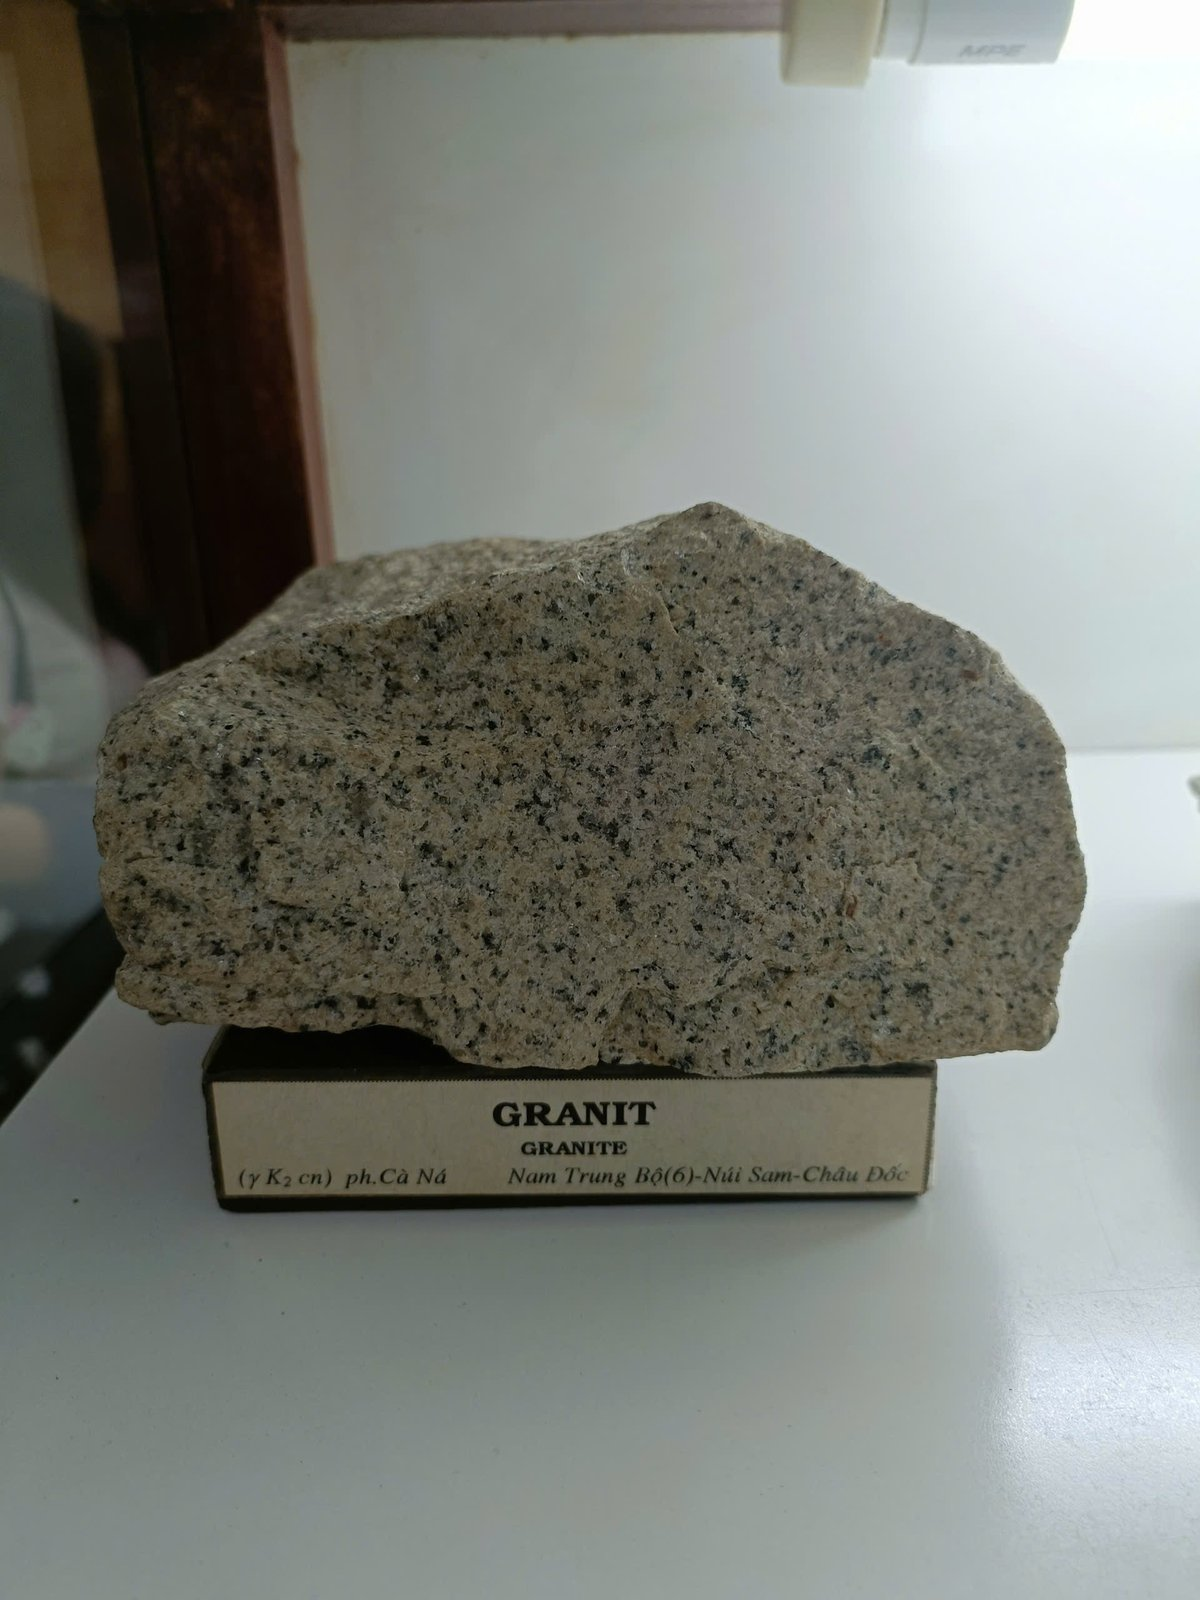
\includegraphics[max width=0.8\linewidth]{graphics/figure_07.jpg}
  \caption{Sample of intrusive igneous rock}
  \label{fig:intrusive-igneous}
\end{figure}

\subsection{Metamorphic process}
\label{subsec:metamorphic-process}

Metamorphism happens when existing rocks undergo high heat, strong pressure, or interaction with reactive fluids, leading them to change into new rock types. At the museum, specimens like schist, gneiss, slate, quartzite, and marble were displayed, each representing different metamorphic environments.

One highlighted example was marble, which develops from limestone through contact metamorphism. The exhibit also included diagrams of metamorphic facies and processes, illustrating how different conditions drive these rock transformations.

\begin{figure}[H]
  \centering
  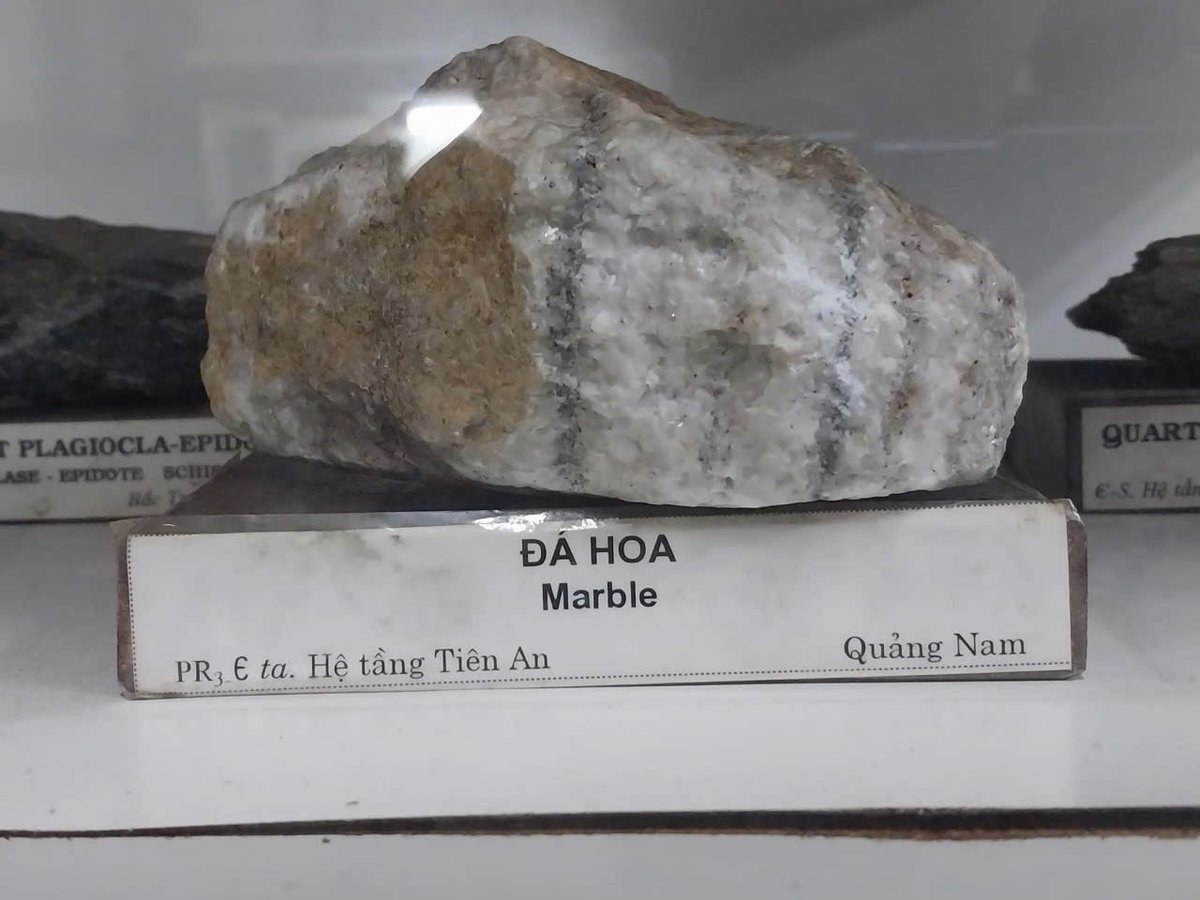
\includegraphics[max width=0.8\linewidth]{graphics/figure_08.jpg}
  \caption{Sample of Marble}
  \label{fig:marble}
\end{figure}

\subsection{Sedimentary process}
\label{subsec:sedimentary-process}

Sedimentary processes occur when materials from older rocks or biological sources are gathered, compressed, and cemented together, resulting in sedimentary rocks that typically show layered structures.

\begin{itemize}
  \item Mechanical sedimentation produces rocks such as sandstone and conglomerate, created from the physical breakdown and accumulation of rock fragments.
  \item Chemical sedimentation is seen in rocks like limestone, which forms when minerals precipitate from water-rich solutions.
\end{itemize}

\begin{figure}[H]
  \centering
  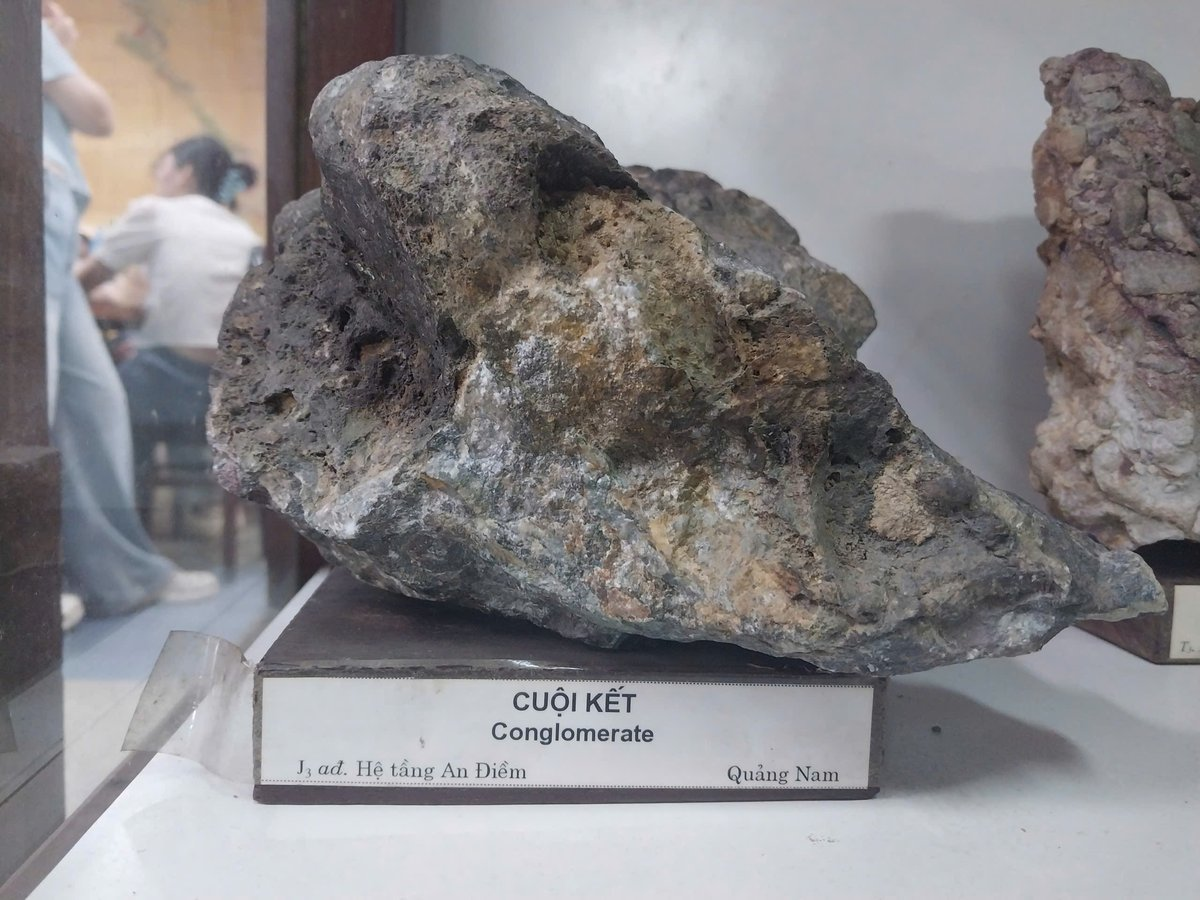
\includegraphics[max width=0.8\linewidth]{graphics/figure_09.jpg}
  \caption{Sample of Mechanical sedimentation rock}
  \label{fig:mechanical-sedimentation}
\end{figure}

\subsection{Weathering process}
\label{subsec:weathering-process}

Weathering is the natural process that breaks down rocks at Earth's surface through the effects of wind, rainfall, temperature changes, and chemical reactions. At the museum, this was demonstrated with diagrams and rock samples that showed how rocks are altered by different types of weathering.

Examples included mechanical weathering, such as rock fragmentation and exfoliation, and chemical weathering, like the oxidation of iron on rock surfaces. These displays highlighted weathering's important role in the rock cycle, as it produces loose sediments that can later compact and cement to form sedimentary rocks.

\begin{figure}[H]
  \centering
  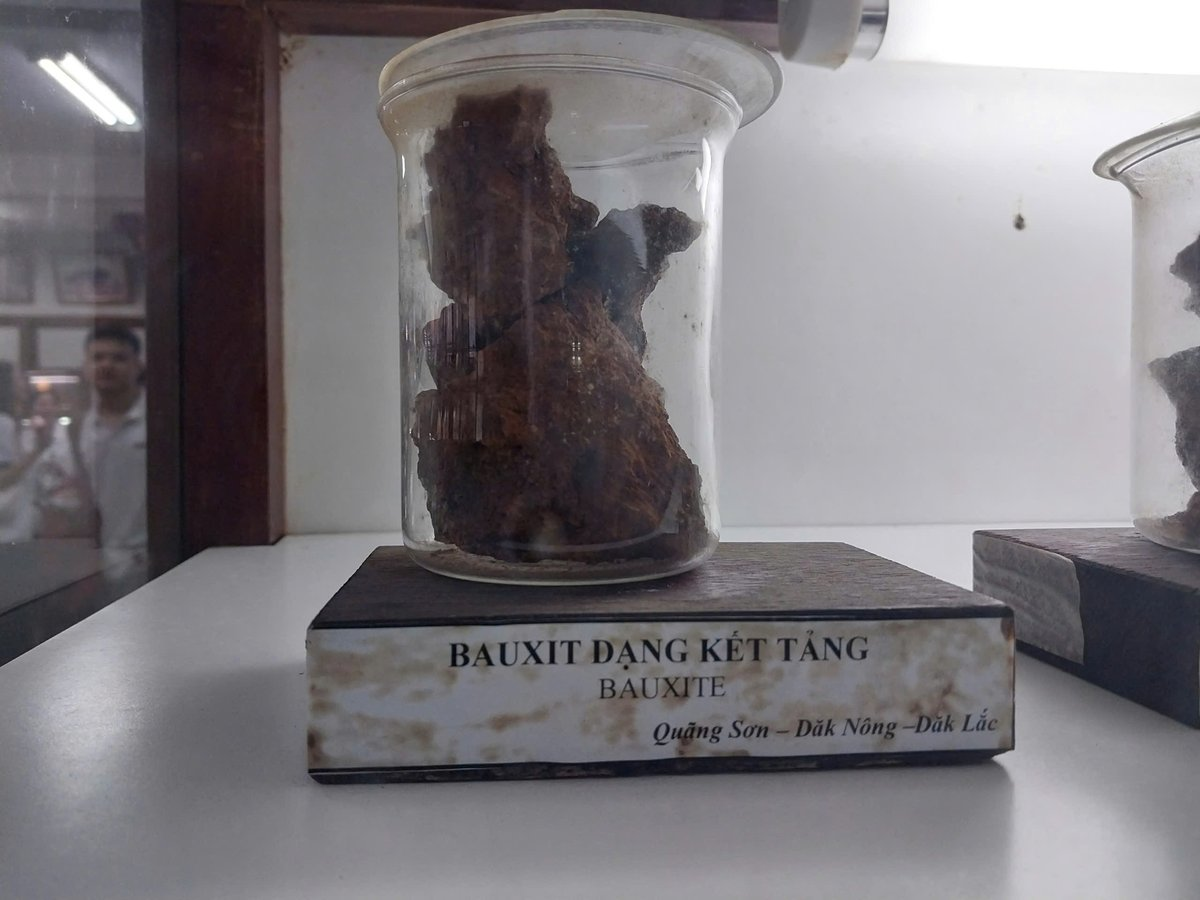
\includegraphics[max width=0.8\linewidth]{graphics/figure_10.jpg}
\caption{Sample of Bauxite}
\label{fig:bauxite}
\end{figure}
\section{MINERAL RESOURCES (2nd floor)}

The second floor of the Ho Chi Minh City Geological Museum showcases Vietnam's abundant mineral wealth and geological resources. This floor provides comprehensive displays of various mineral categories, from energy resources to precious gemstones, offering visitors insight into the country's geological diversity and economic potential. The exhibits demonstrate how these natural resources have been formed through millions of years of geological processes and their significance to Vietnam's development.

\subsection{Energy and Fuel Resources}

Energy resources represent naturally occurring materials that can be utilized to generate power and heat through combustion or other processes. The museum's collection highlights two fundamental categories of fossil fuels that have shaped Vietnam's energy landscape.

\textbf{Petroleum} constitutes a crucial liquid hydrocarbon resource formed from ancient marine organisms subjected to heat and pressure over geological time scales. This valuable resource undergoes refining processes to produce essential fuels including gasoline, diesel fuel, and aviation kerosene. Vietnam's petroleum reserves, particularly in offshore basins, play a vital role in the nation's energy security and economic development.

\begin{figure}[H]
\centering
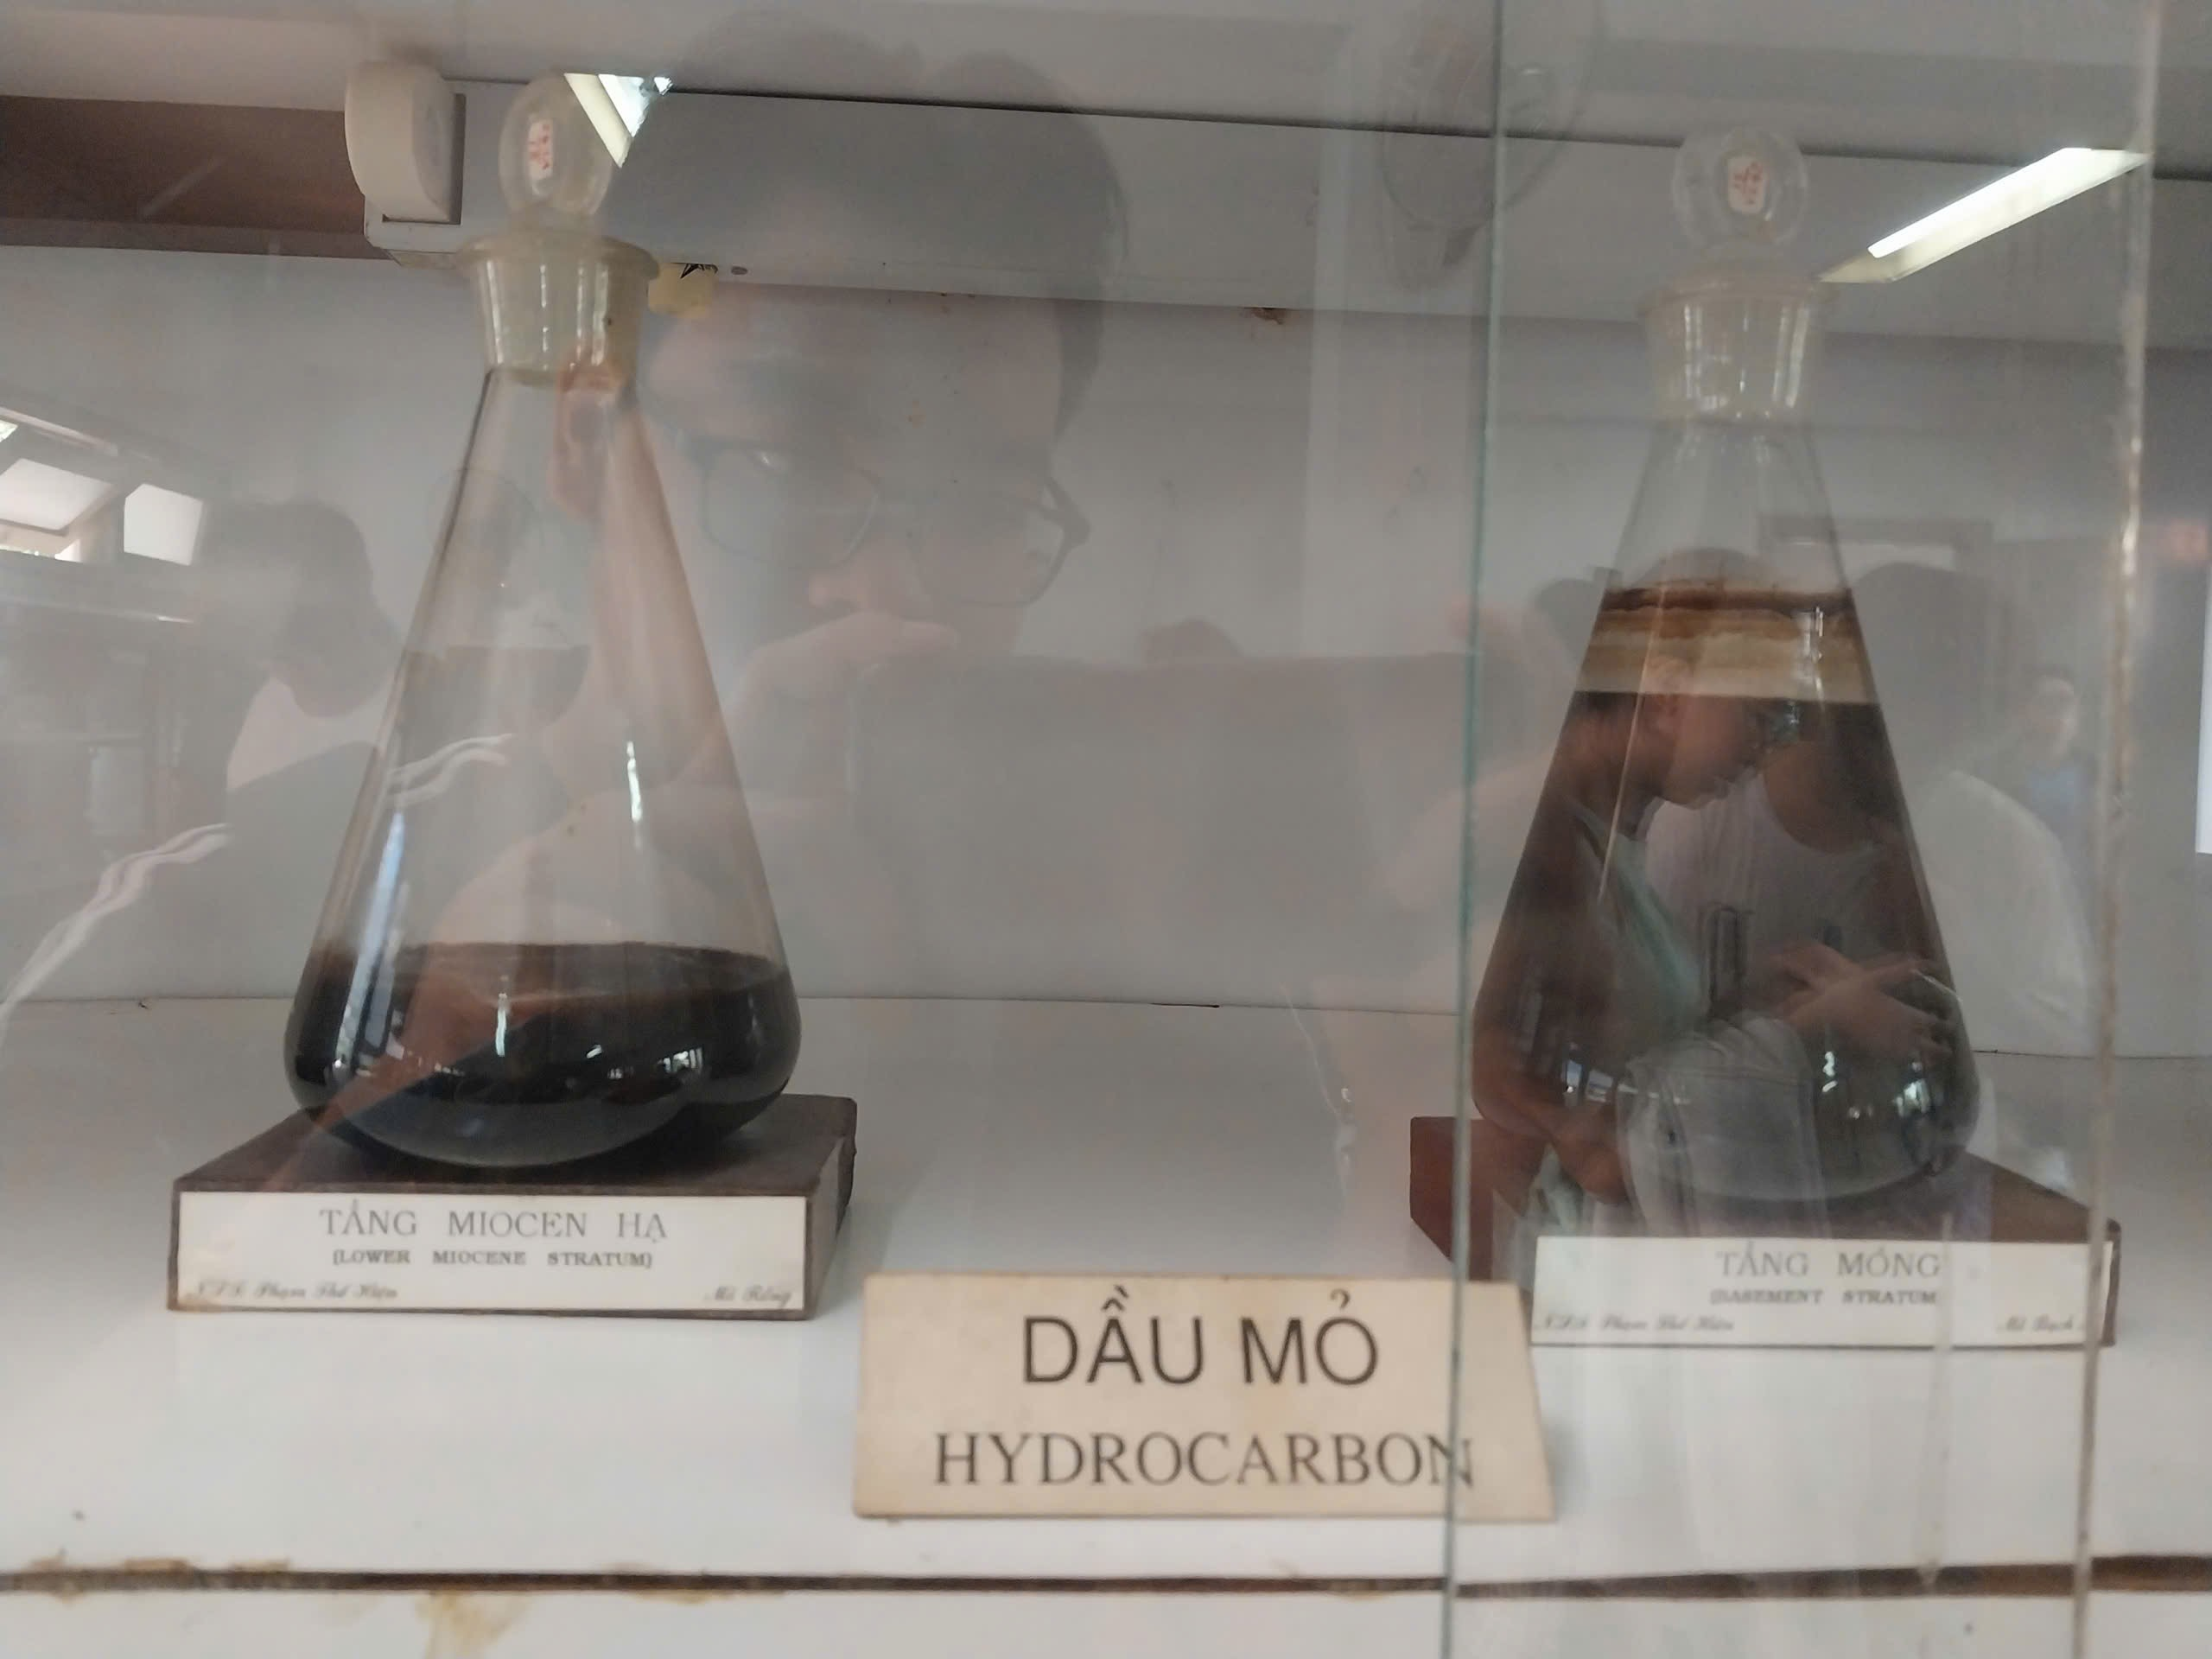
\includegraphics[width=0.7\textwidth]{graphics/petroleum_sample.png}
\caption{Petroleum sample display from Vietnamese offshore reserves}
\label{fig:petroleum}
\end{figure}

\textbf{Coal} represents a solid fossil fuel derived from ancient plant matter that underwent transformation through geological compression and heating over millions of years. The museum displays various coal types classified by their carbon content and energy density:
\begin{itemize}
    \item Peat -- representing the earliest stage of coal development
    \item Lignite -- commonly referred to as brown coal with moderate energy content
    \item Bituminous coal -- a widely utilized intermediate-grade coal
    \item Anthracite -- the highest quality coal with maximum energy output
\end{itemize}

\begin{figure}[H]
\centering
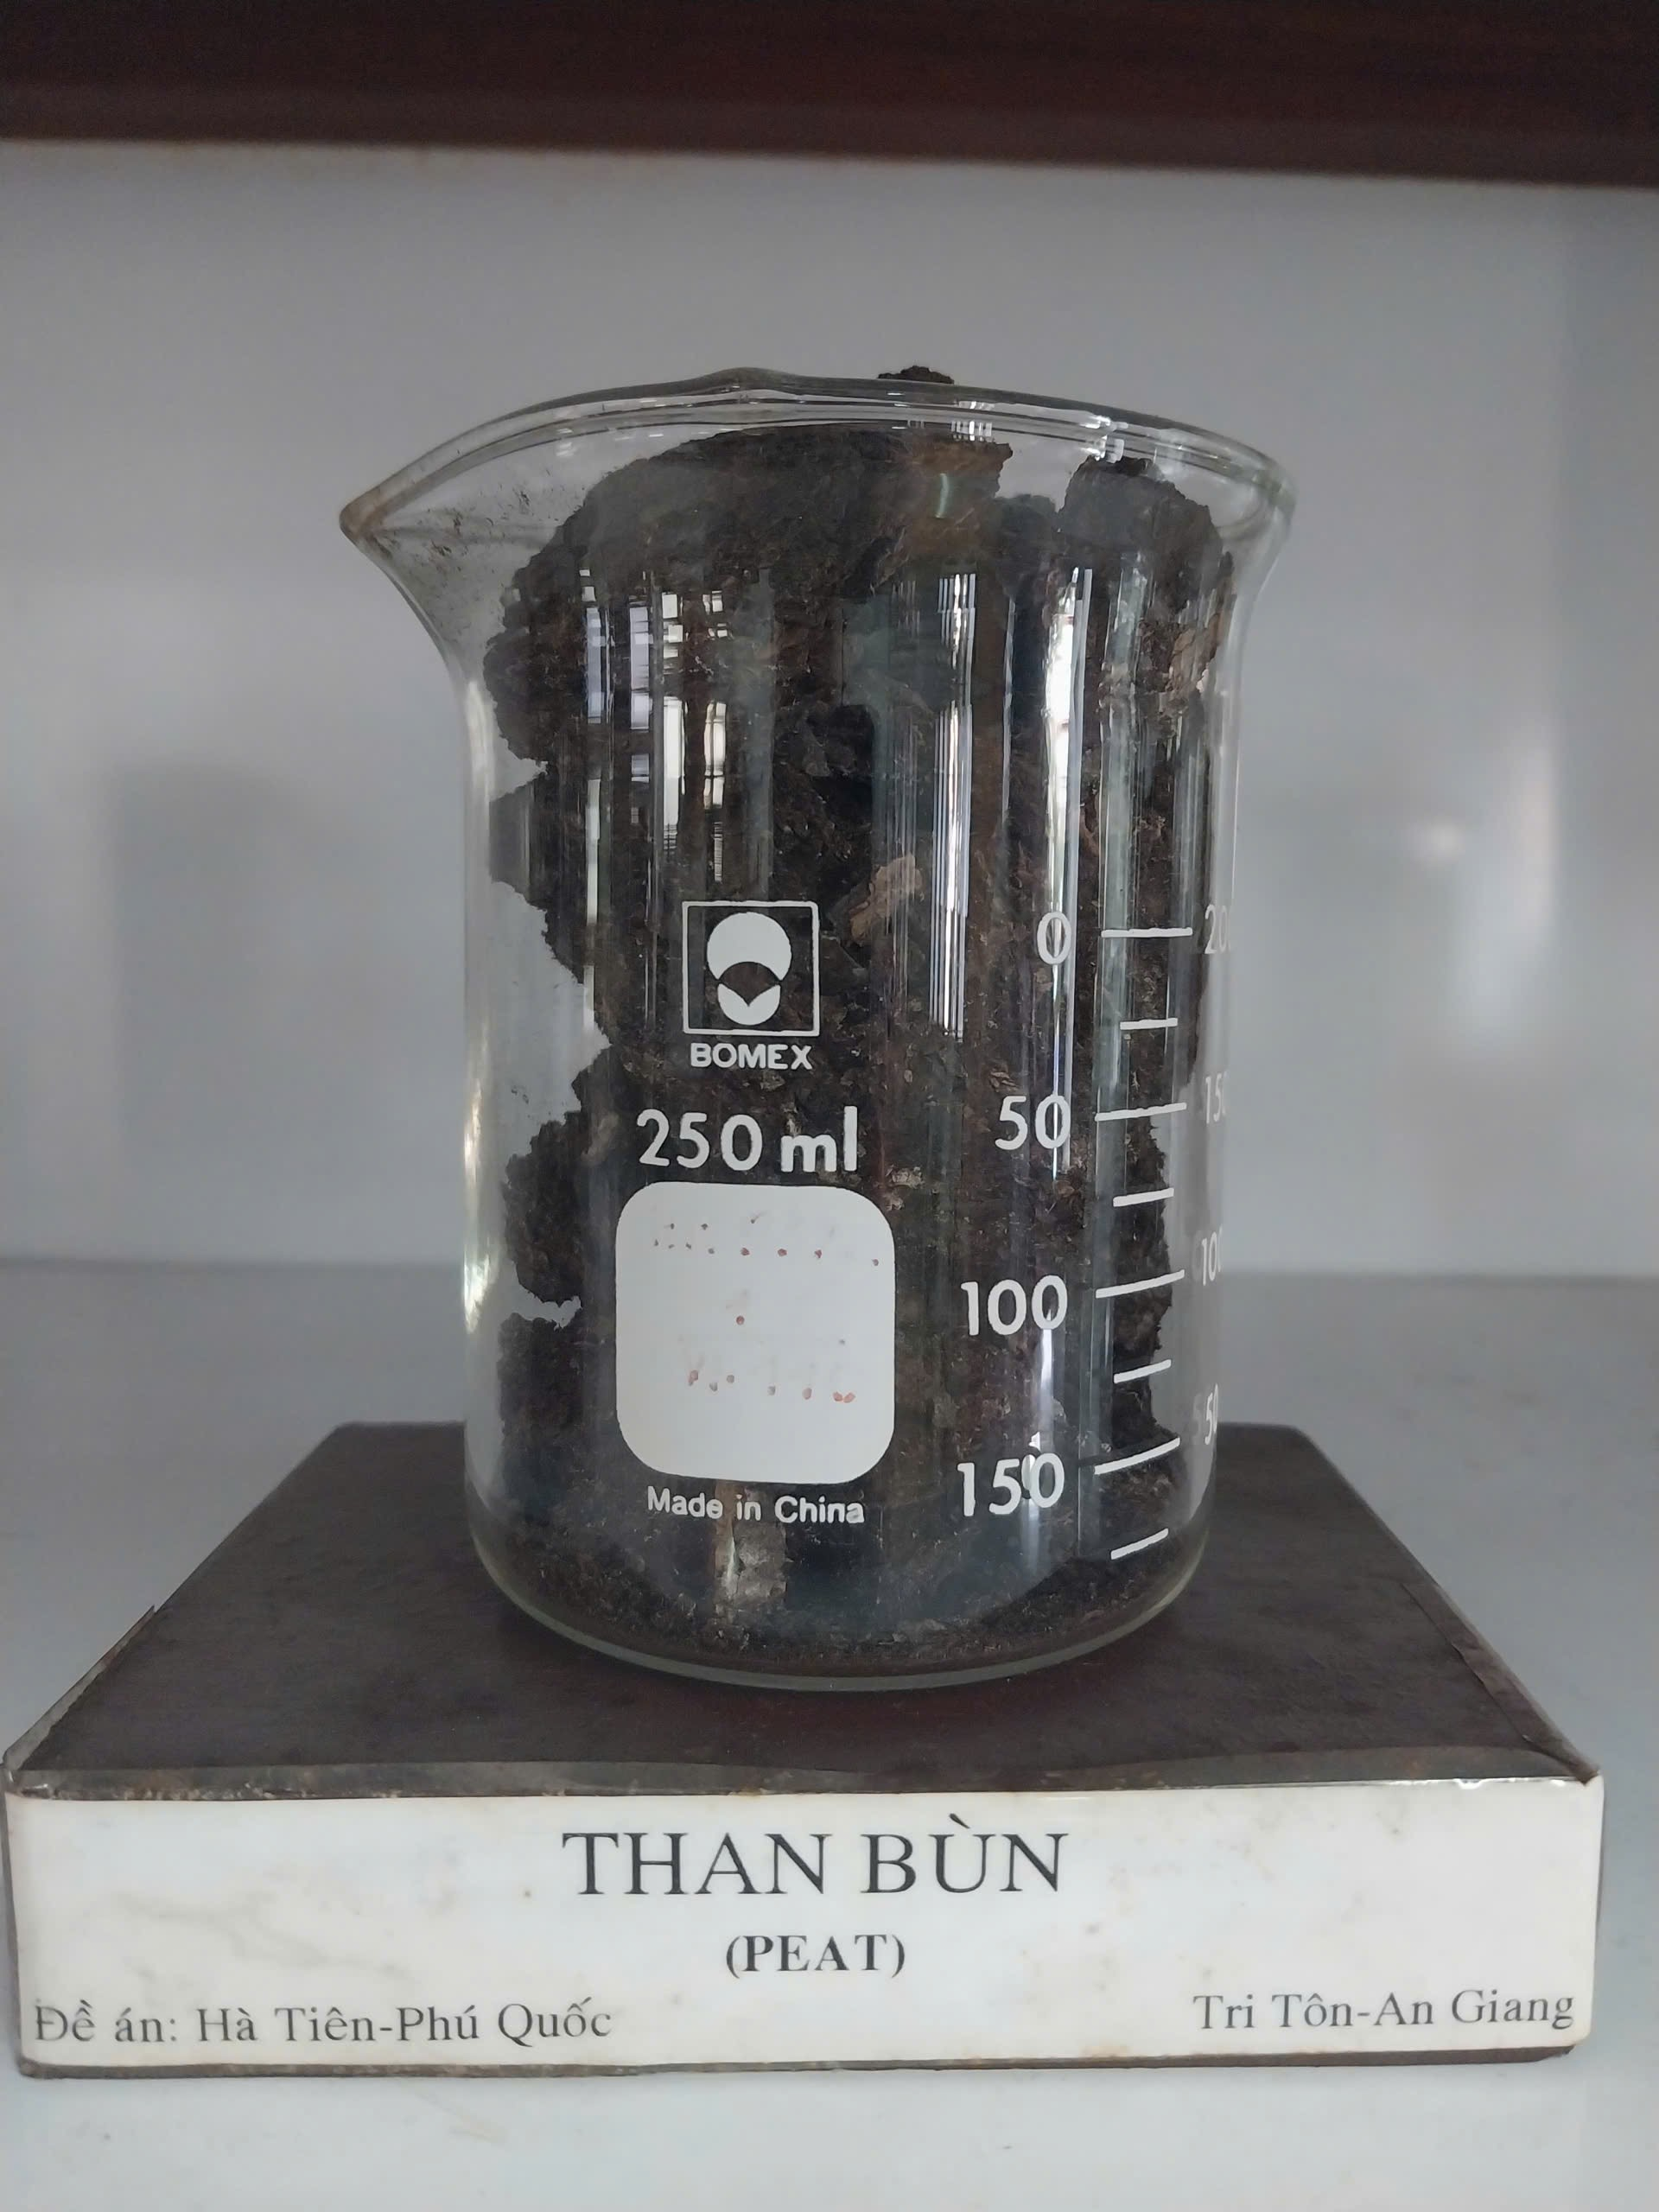
\includegraphics[width=0.7\textwidth]{graphics/coal_types.png}
\caption{Different types of coal samples showing progression from peat to anthracite}
\label{fig:coal_types}
\end{figure}

These coal varieties serve primarily in electrical power generation and industrial applications, including steel production processes.

\begin{figure}[H]
\centering
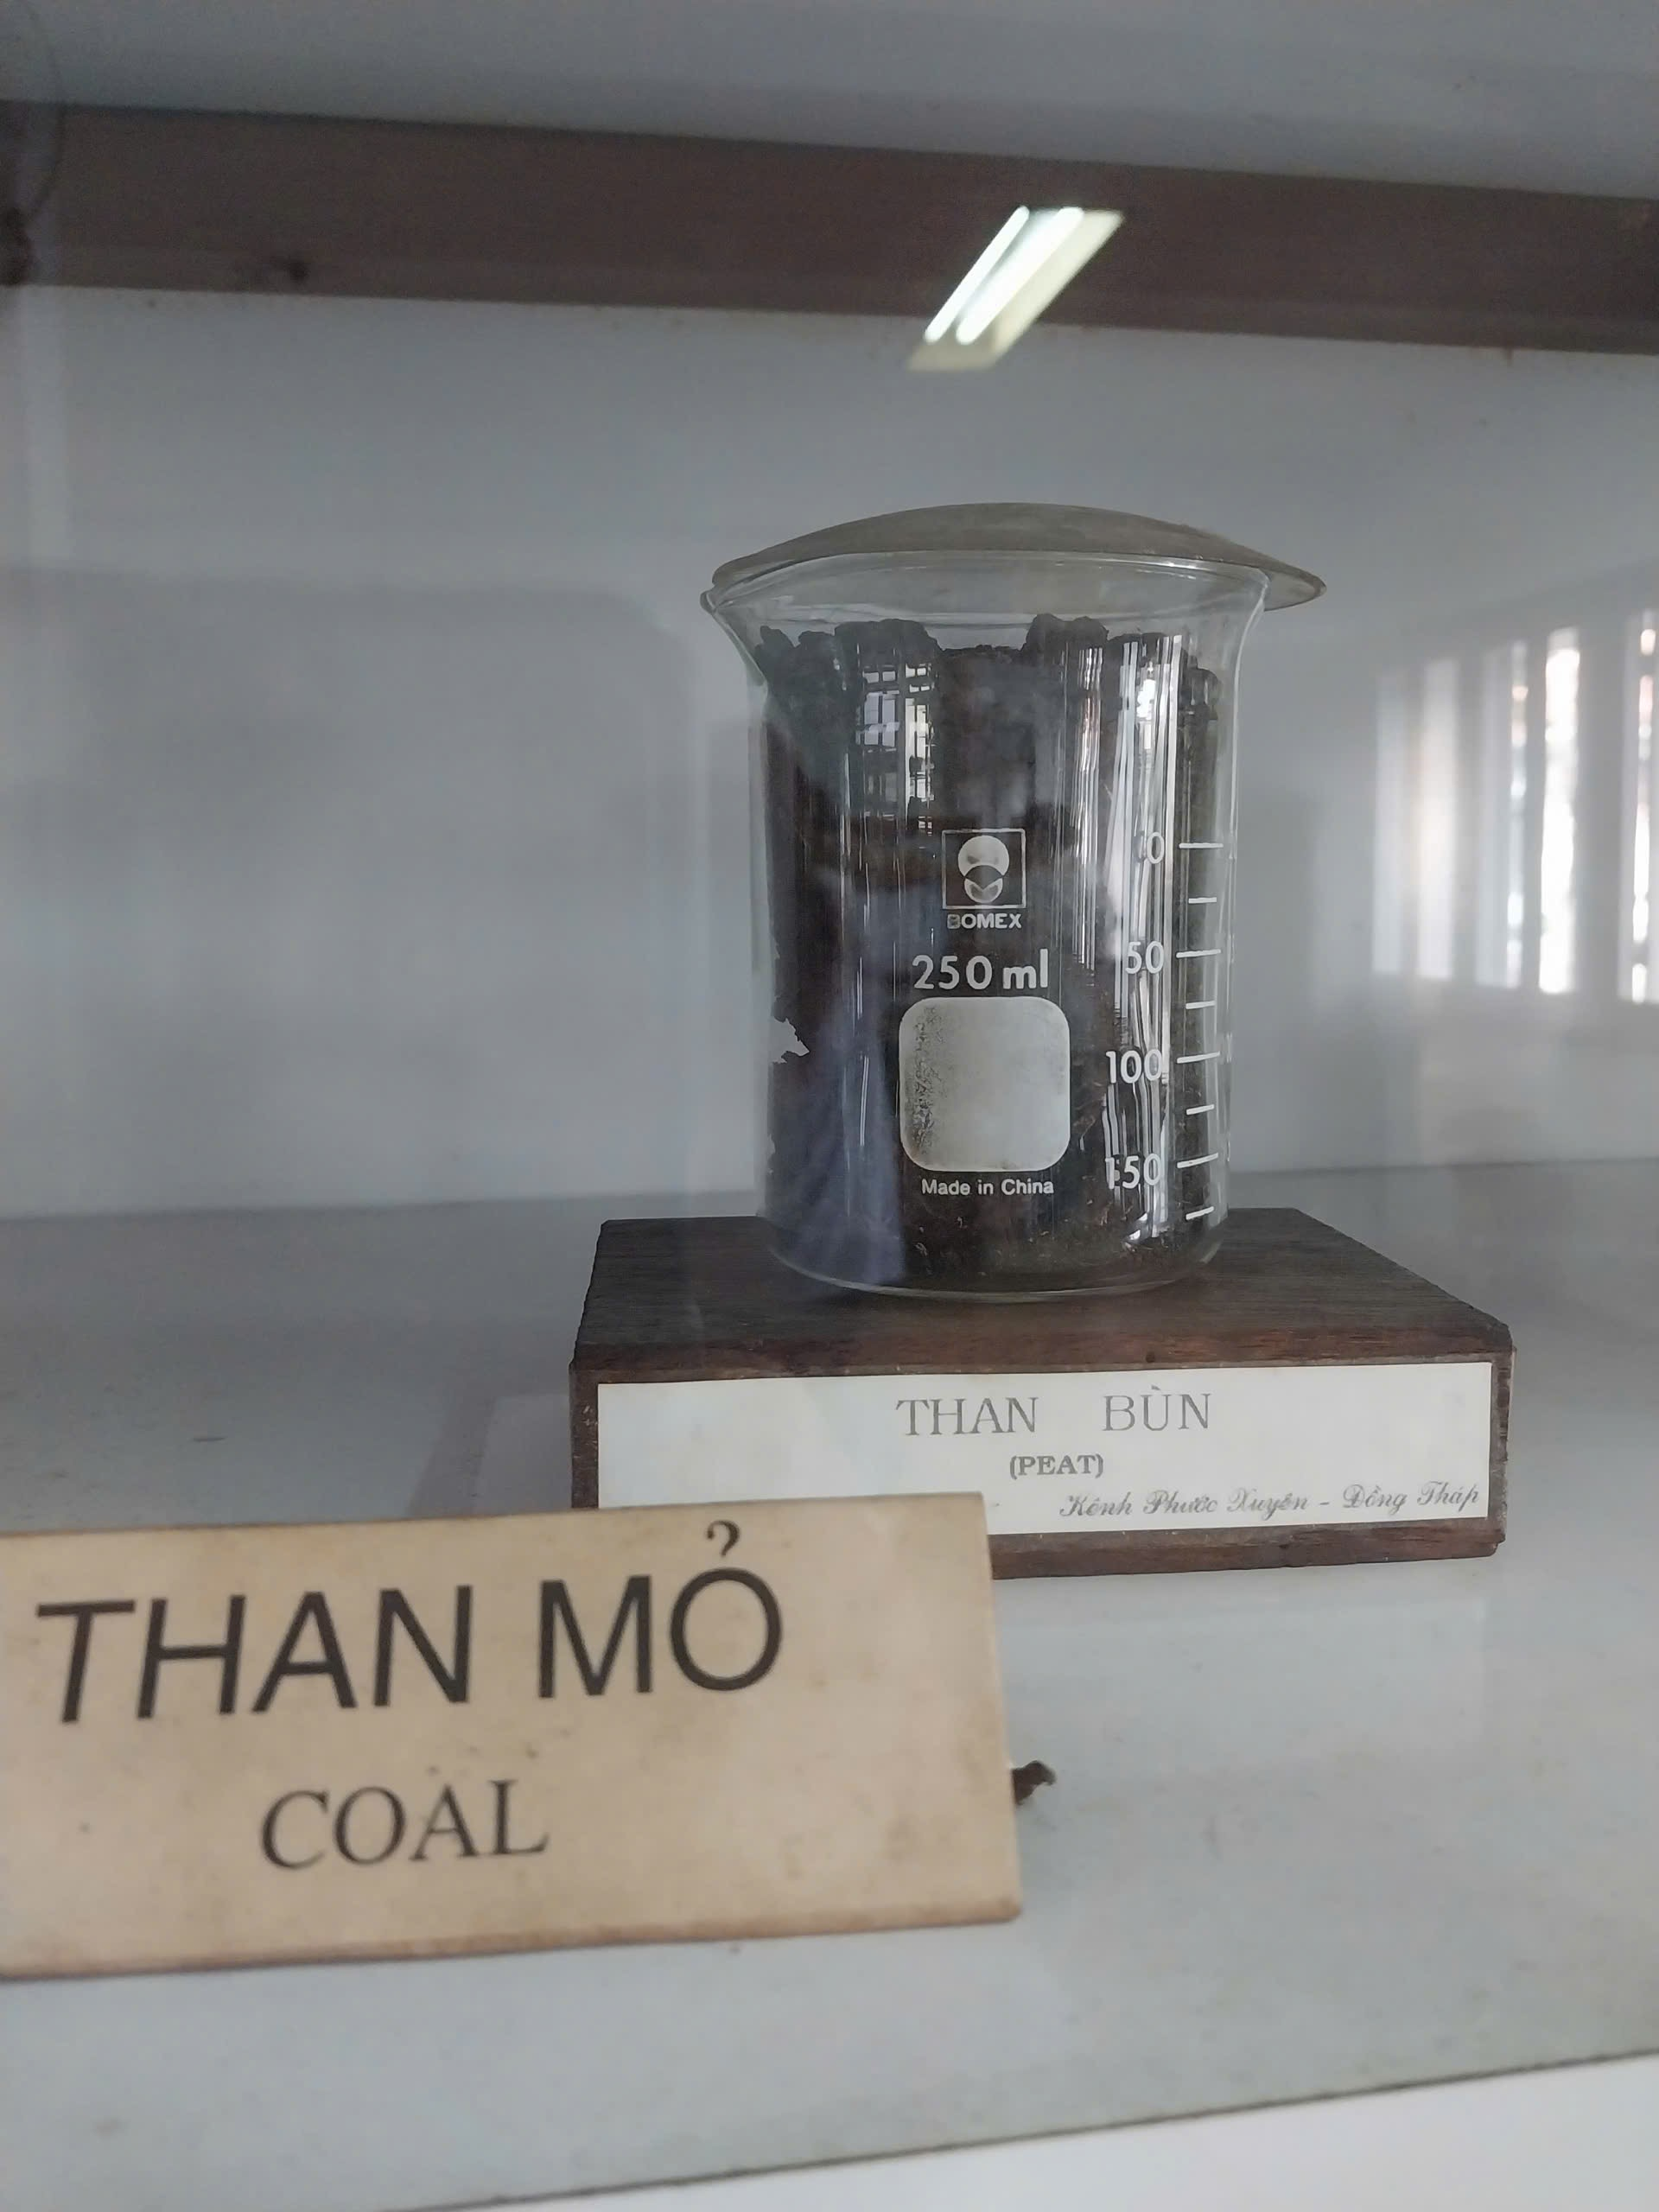
\includegraphics[width=0.7\textwidth]{graphics/coal_types_2.png}
\caption{Additional coal specimens from Vietnamese geological formations}
\label{fig:coal_specimens}
\end{figure}

\subsection{Metallic Mineral Resources}

Vietnam possesses diverse metallic mineral resources distributed across different geological regions.

\textbf{Strategic Metals}
\textit{Titanium:} A lightweight, strong, and corrosion-resistant metal used in aerospace and medical applications. Vietnam has titanium deposits primarily in coastal sand formations.

\textit{Tin:} Vietnam is one of the world's significant tin producers, with major deposits in the northern provinces. Tin is essential for electronics and soldering applications.

\textit{Chromium:} Used in stainless steel production and chrome plating. Vietnam's chromium deposits are found in ultramafic rock formations.

\textit{Rare Earth Elements:} Critical for modern technology including electronics, renewable energy systems, and defense applications.

\begin{figure}[H]
\centering
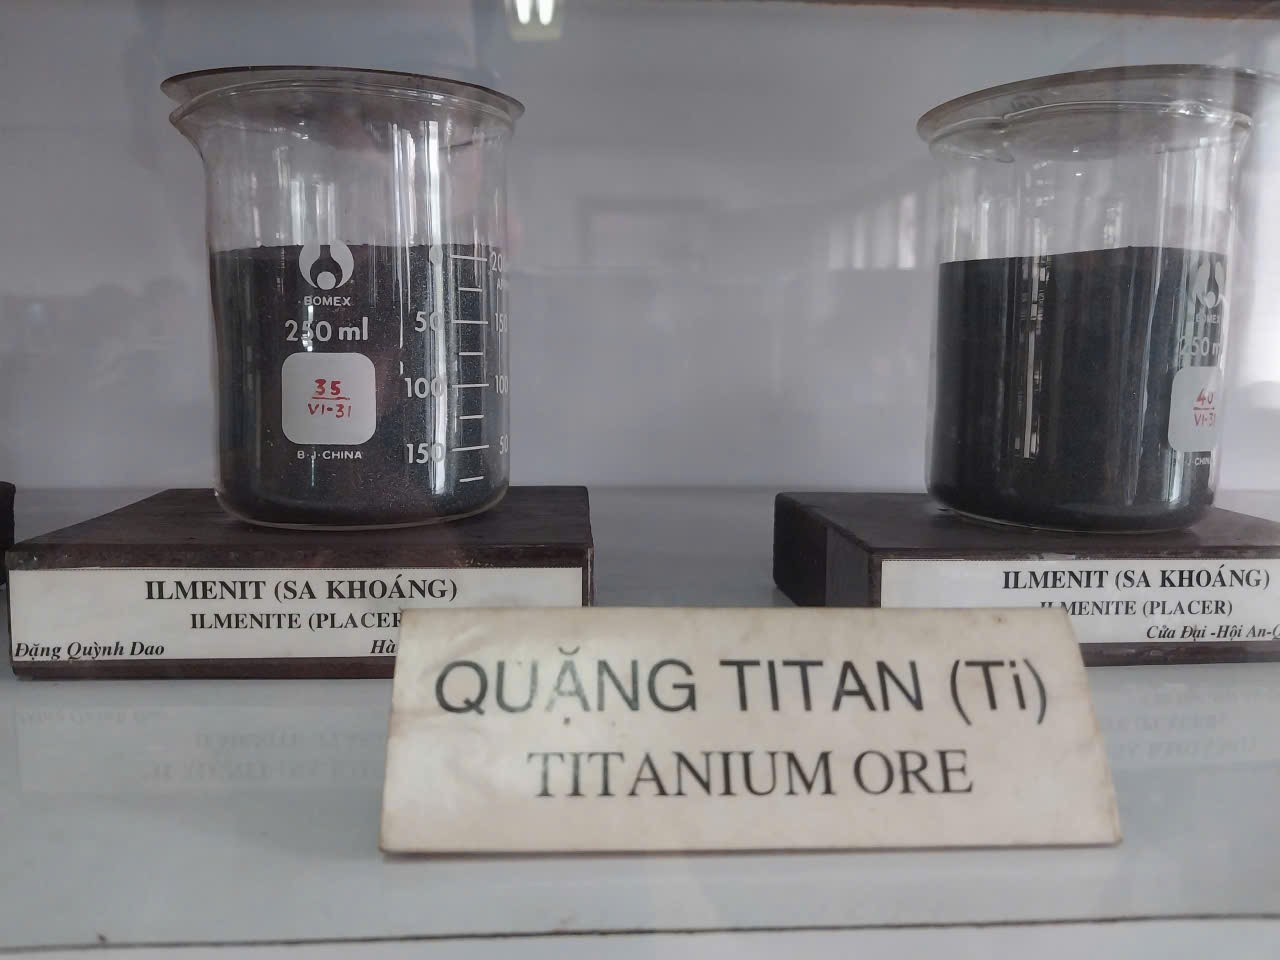
\includegraphics[width=0.7\textwidth]{graphics/strategic_metals.png}
\caption{Strategic metal samples including titanium and rare earth elements}
\label{fig:strategic_metals}
\end{figure}

\textbf{Industrial Metals}
\textit{Iron:} The foundation of steel production, Vietnam has significant iron ore deposits in the northern regions, particularly in Thai Nguyen and Lao Cai provinces.

\textit{Aluminum:} Derived from bauxite ore, Vietnam has substantial bauxite reserves in the Central Highlands region.

\textit{Copper:} Essential for electrical applications and construction. Vietnam's copper deposits are found in various geological formations.

\textit{Zinc:} Used in galvanizing and alloy production. Vietnam has zinc deposits associated with lead mineralization.

\textit{Lead:} Important for batteries and radiation shielding applications.

\begin{figure}[H]
\centering
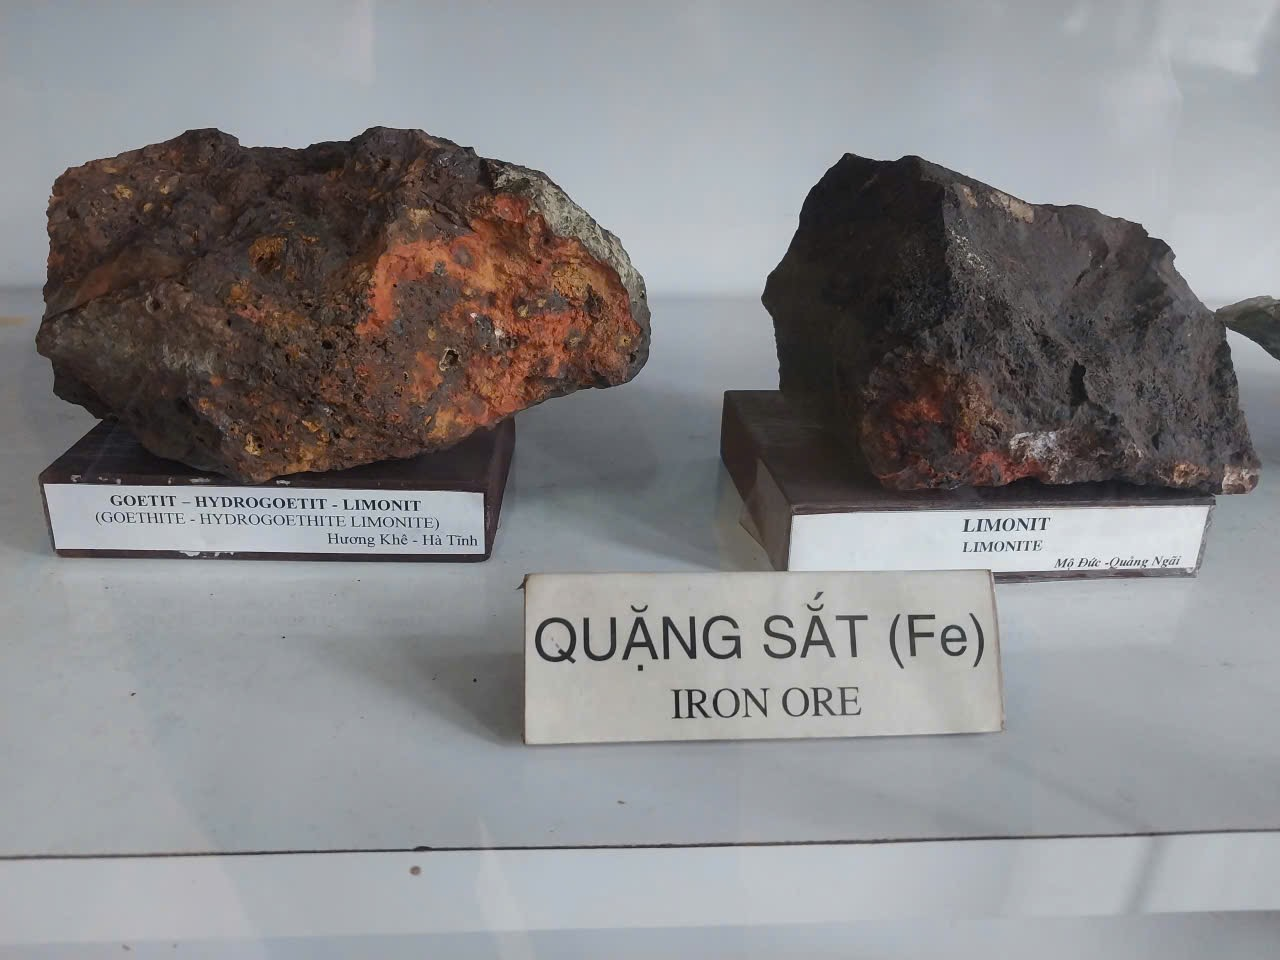
\includegraphics[width=0.7\textwidth]{graphics/industrial_metals.png}
\caption{Industrial metal samples including iron ore and copper}
\label{fig:industrial_metals}
\end{figure}

\textbf{Precious Metals}
\textit{Gold:} Vietnam has both placer and lode gold deposits. Gold mining has a long history in Vietnam, with significant deposits in Quang Nam and other provinces.

\textit{Silver:} Often found associated with other metal ores, silver has both monetary and industrial applications.

\begin{figure}[H]
\centering
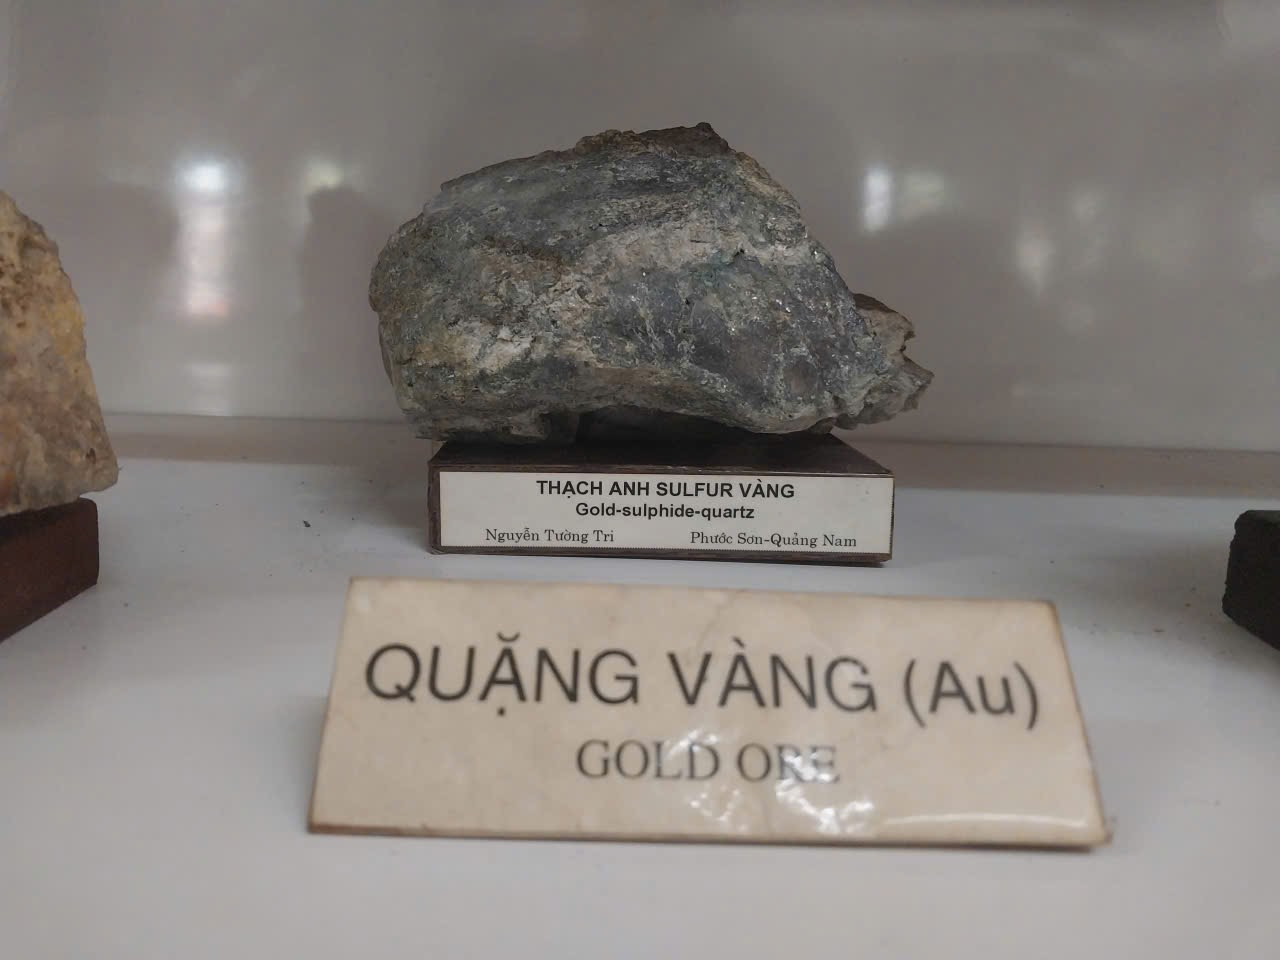
\includegraphics[width=0.7\textwidth]{graphics/precious_metals.png}
\caption{Gold and silver samples from Vietnamese deposits}
\label{fig:precious_metals}
\end{figure}

\textbf{Specialty Metals}
\textit{Tungsten:} Vietnam is a major tungsten producer globally. Tungsten is essential for high-temperature applications and cutting tools.

\textit{Molybdenum:} Used in steel alloys and high-temperature applications.

\textit{Magnesium:} Lightweight metal used in aerospace and automotive industries.

\subsection{Non-Metallic Mineral Resources}

Non-metallic minerals represent naturally occurring substances lacking metallic properties but possessing significant industrial and economic value. These materials serve essential functions in construction, agriculture, and manufacturing sectors.

\textbf{Silica Sand}
High-purity silica sand is essential for glass manufacturing, foundry operations, and construction applications. Vietnam has significant silica sand deposits along its coastal regions, particularly suitable for high-quality glass production.


\textbf{Pyrite}
Iron sulfide mineral (FeS₂) with applications in sulfuric acid production and as a source of sulfur for chemical industries. Pyrite is also known as "fool's gold" due to its metallic luster and golden color.

\begin{figure}[H]
\centering
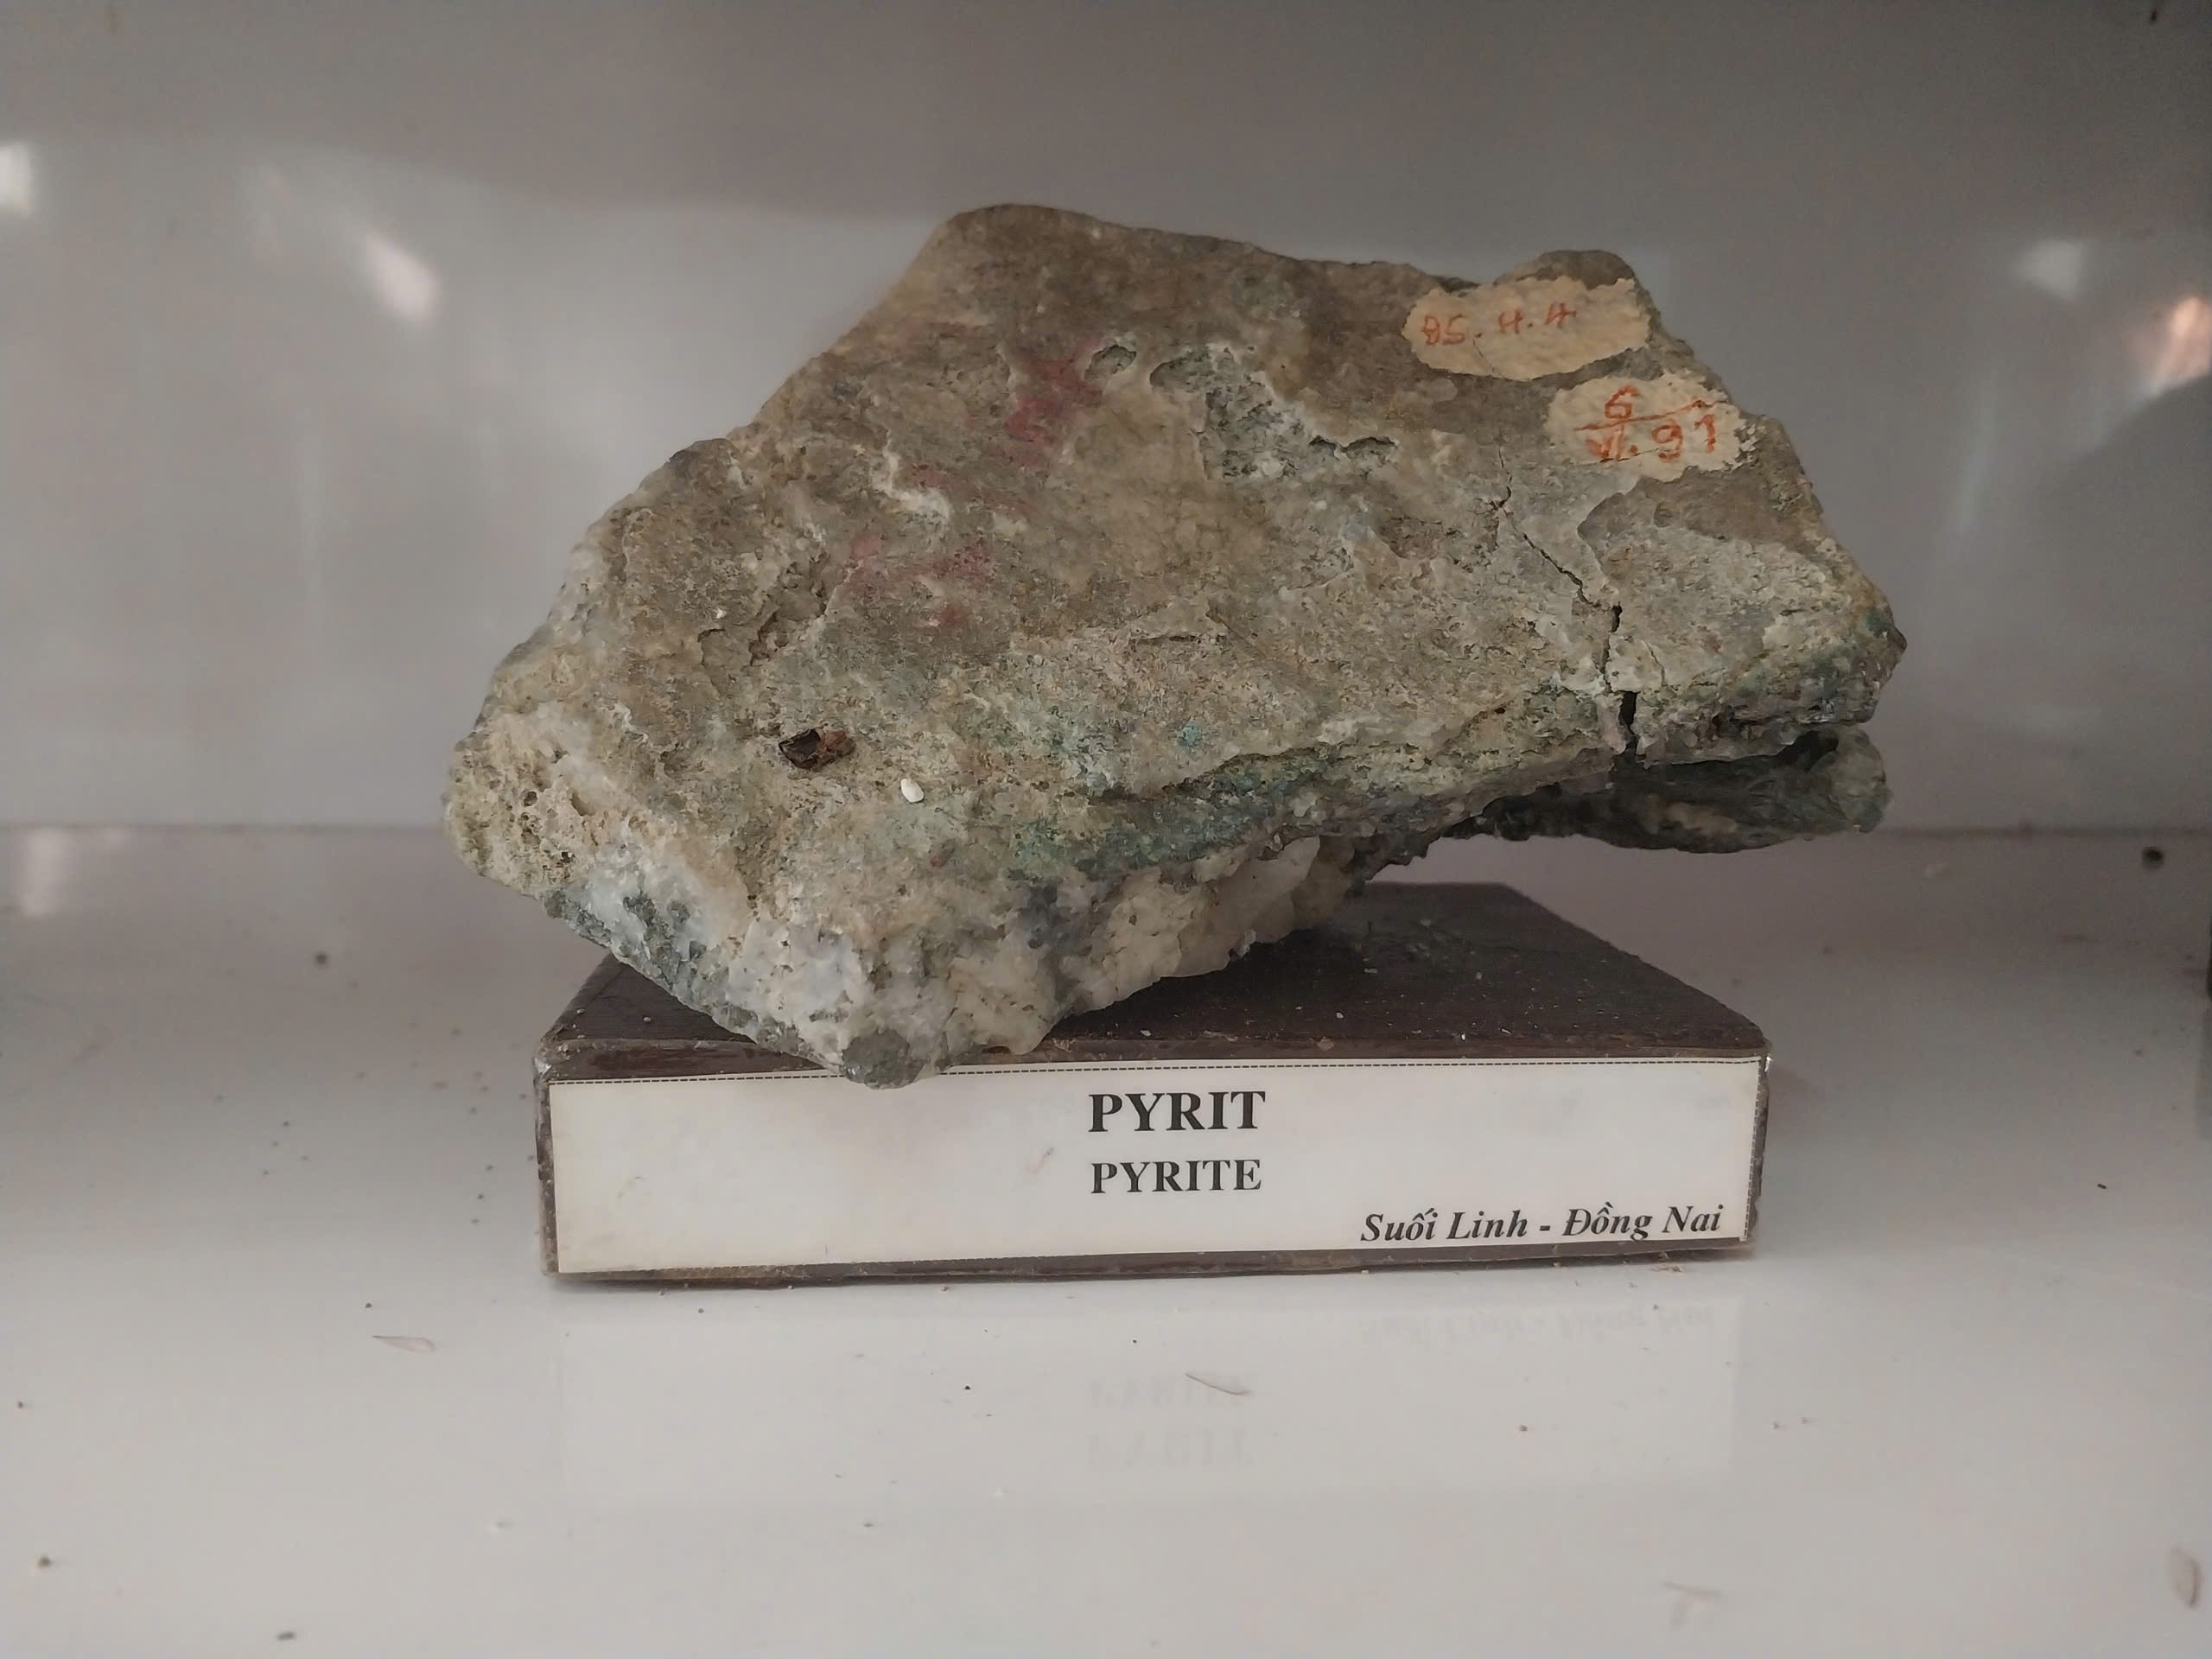
\includegraphics[width=0.7\textwidth]{graphics/pyrite.png}
\caption{Pyrite specimen showing characteristic metallic luster}
\label{fig:pyrite}
\end{figure}

\textbf{Apatite}
Phosphate mineral essential for fertilizer production and chemical industries. Vietnam has significant apatite deposits that support the country's agricultural sector through phosphate fertilizer production.

\textbf{Talc}
A soft silicate mineral used in cosmetics, paper, paint, and ceramic industries due to its lubricating properties and chemical inertness.

\textbf{Asbestos}
Fibrous silicate minerals with heat-resistant properties, though their use is now restricted due to health concerns.

\textbf{Phosphorite}
Sedimentary rock containing phosphate minerals, primarily used for fertilizer production.

\textbf{Kaolin}
A fine clay mineral used in ceramics, paper production, and as a filler in various industrial applications.

\subsection{Construction Materials}

Construction materials encompass naturally occurring substances utilized in building and infrastructure development. These materials form the foundation of human civilization's architectural achievements and continue to play crucial roles in modern construction practices.

\textbf{Stone Materials}
\textit{Limestone:} Sedimentary rock composed primarily of calcium carbonate, essential for cement production and construction. Vietnam has extensive limestone deposits throughout the country.

\textit{Marble:} Metamorphosed limestone prized for decorative applications and high-end construction projects. Vietnamese marble is known for its quality and diverse colors.

\textit{Granite:} Igneous rock valued for its durability and aesthetic appeal in construction and monuments. Vietnam has significant granite quarries producing various colors and textures.

\begin{figure}[H]
\centering
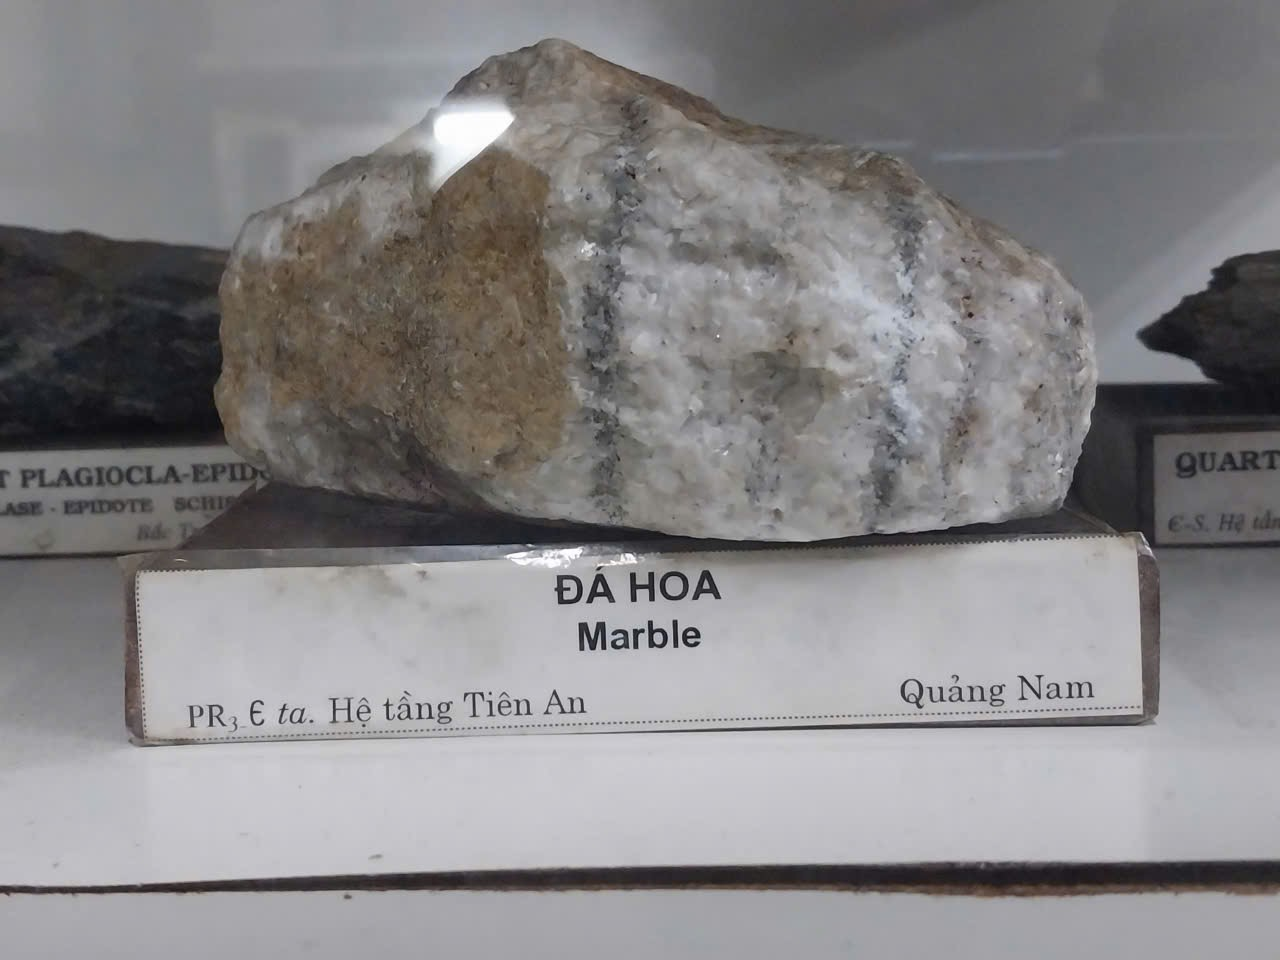
\includegraphics[width=0.7\textwidth]{graphics/stone_materials.png}
\caption{Marble sample}
\label{fig:stone_materials}
\end{figure}

\textbf{Clay and Ceramic Materials}
\textit{Clay:} Fine-grained sedimentary material essential for brick, tile, and ceramic production. Vietnam has abundant clay deposits suitable for various ceramic applications.

\textit{Kaolin:} High-quality white clay used in fine ceramics and porcelain production.


\textbf{Aggregate Materials}
\textit{Sand:} Essential component for concrete production and construction applications. Vietnam has both river sand and marine sand resources.

\textit{Gravel:} Coarse aggregate material used in concrete and road construction.

\textit{Crushed Stone:} Processed stone aggregate for various construction applications.

\begin{figure}[H]
    \centering
    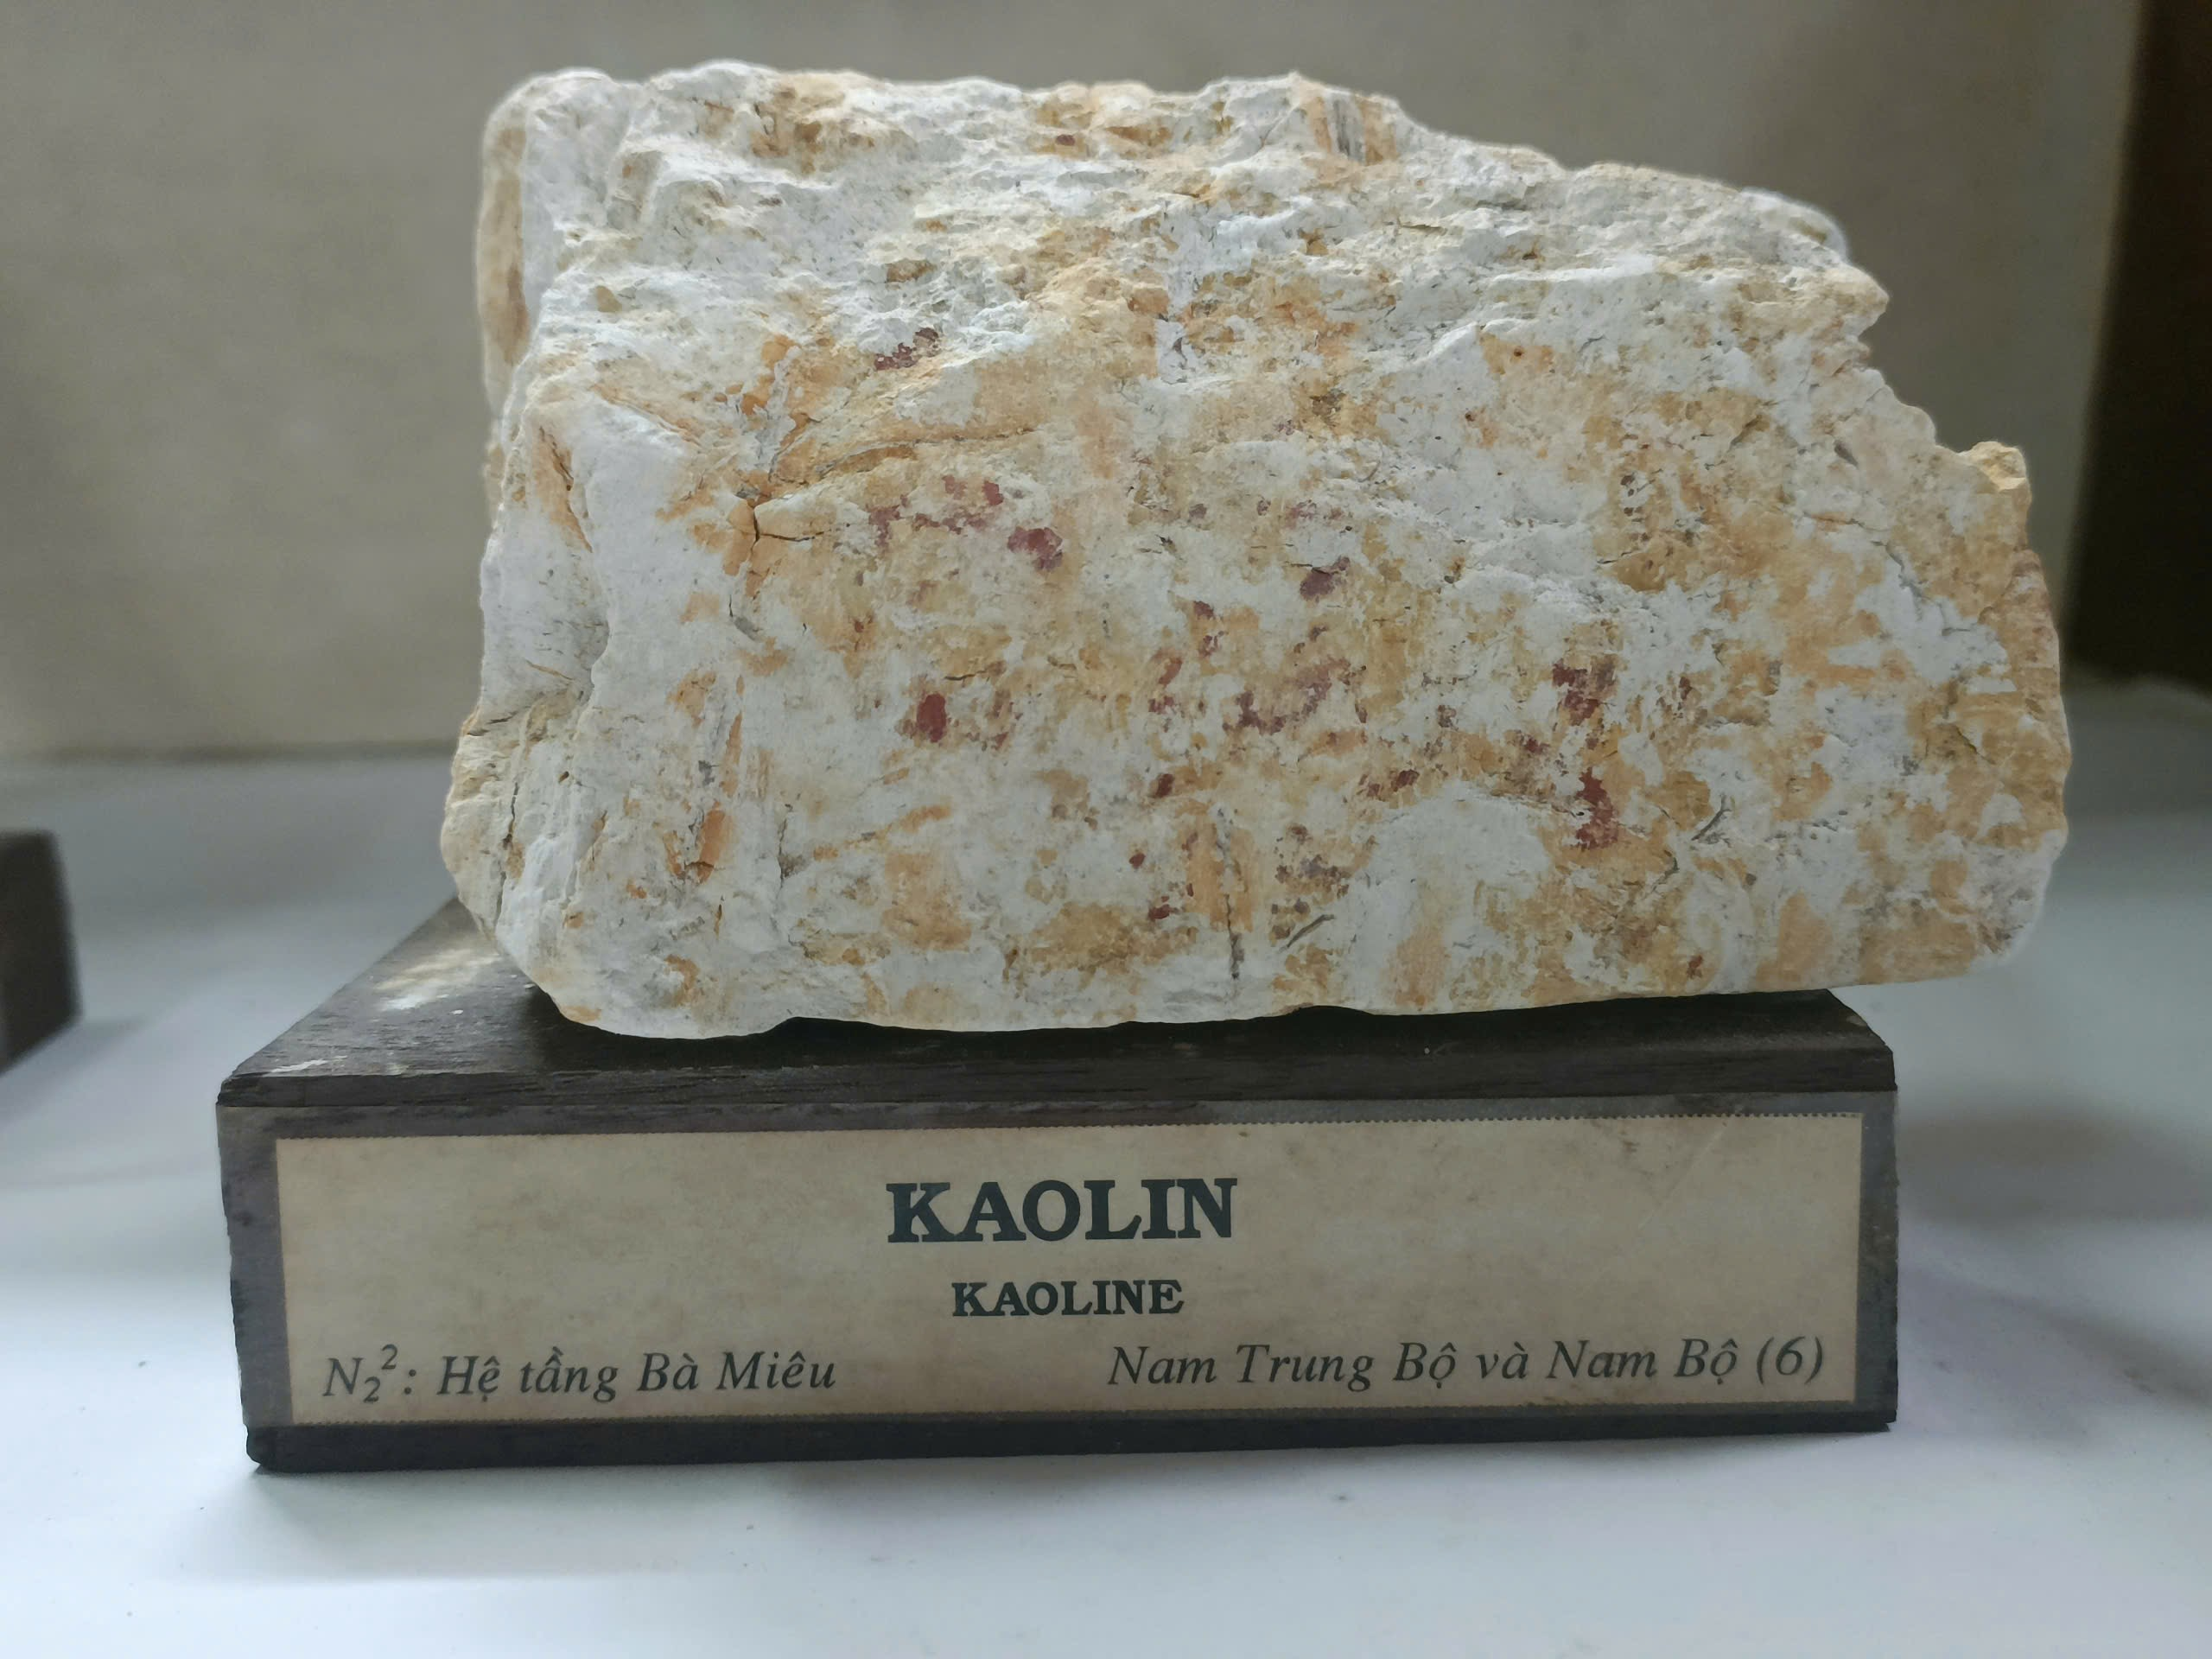
\includegraphics[width=0.7\textwidth]{graphics/kaolin_clay.png}
    \caption{Kaolin clay sample showing characteristic white coloration and fine texture}
    \label{fig:kaolin_clay}
\end{figure}

\subsection{Gemstones and Semi-Precious Stones}

Vietnam possesses notable gemstone deposits with both aesthetic and economic value.

\textbf{Quartz Varieties}
\textit{Amethyst:} A purple variety of quartz that is highly prized for jewelry and decorative purposes. The purple color comes from trace amounts of iron and aluminum impurities. Amethyst is found in various locations throughout Vietnam and is considered one of the most valuable quartz varieties.

\begin{figure}[H]
\centering
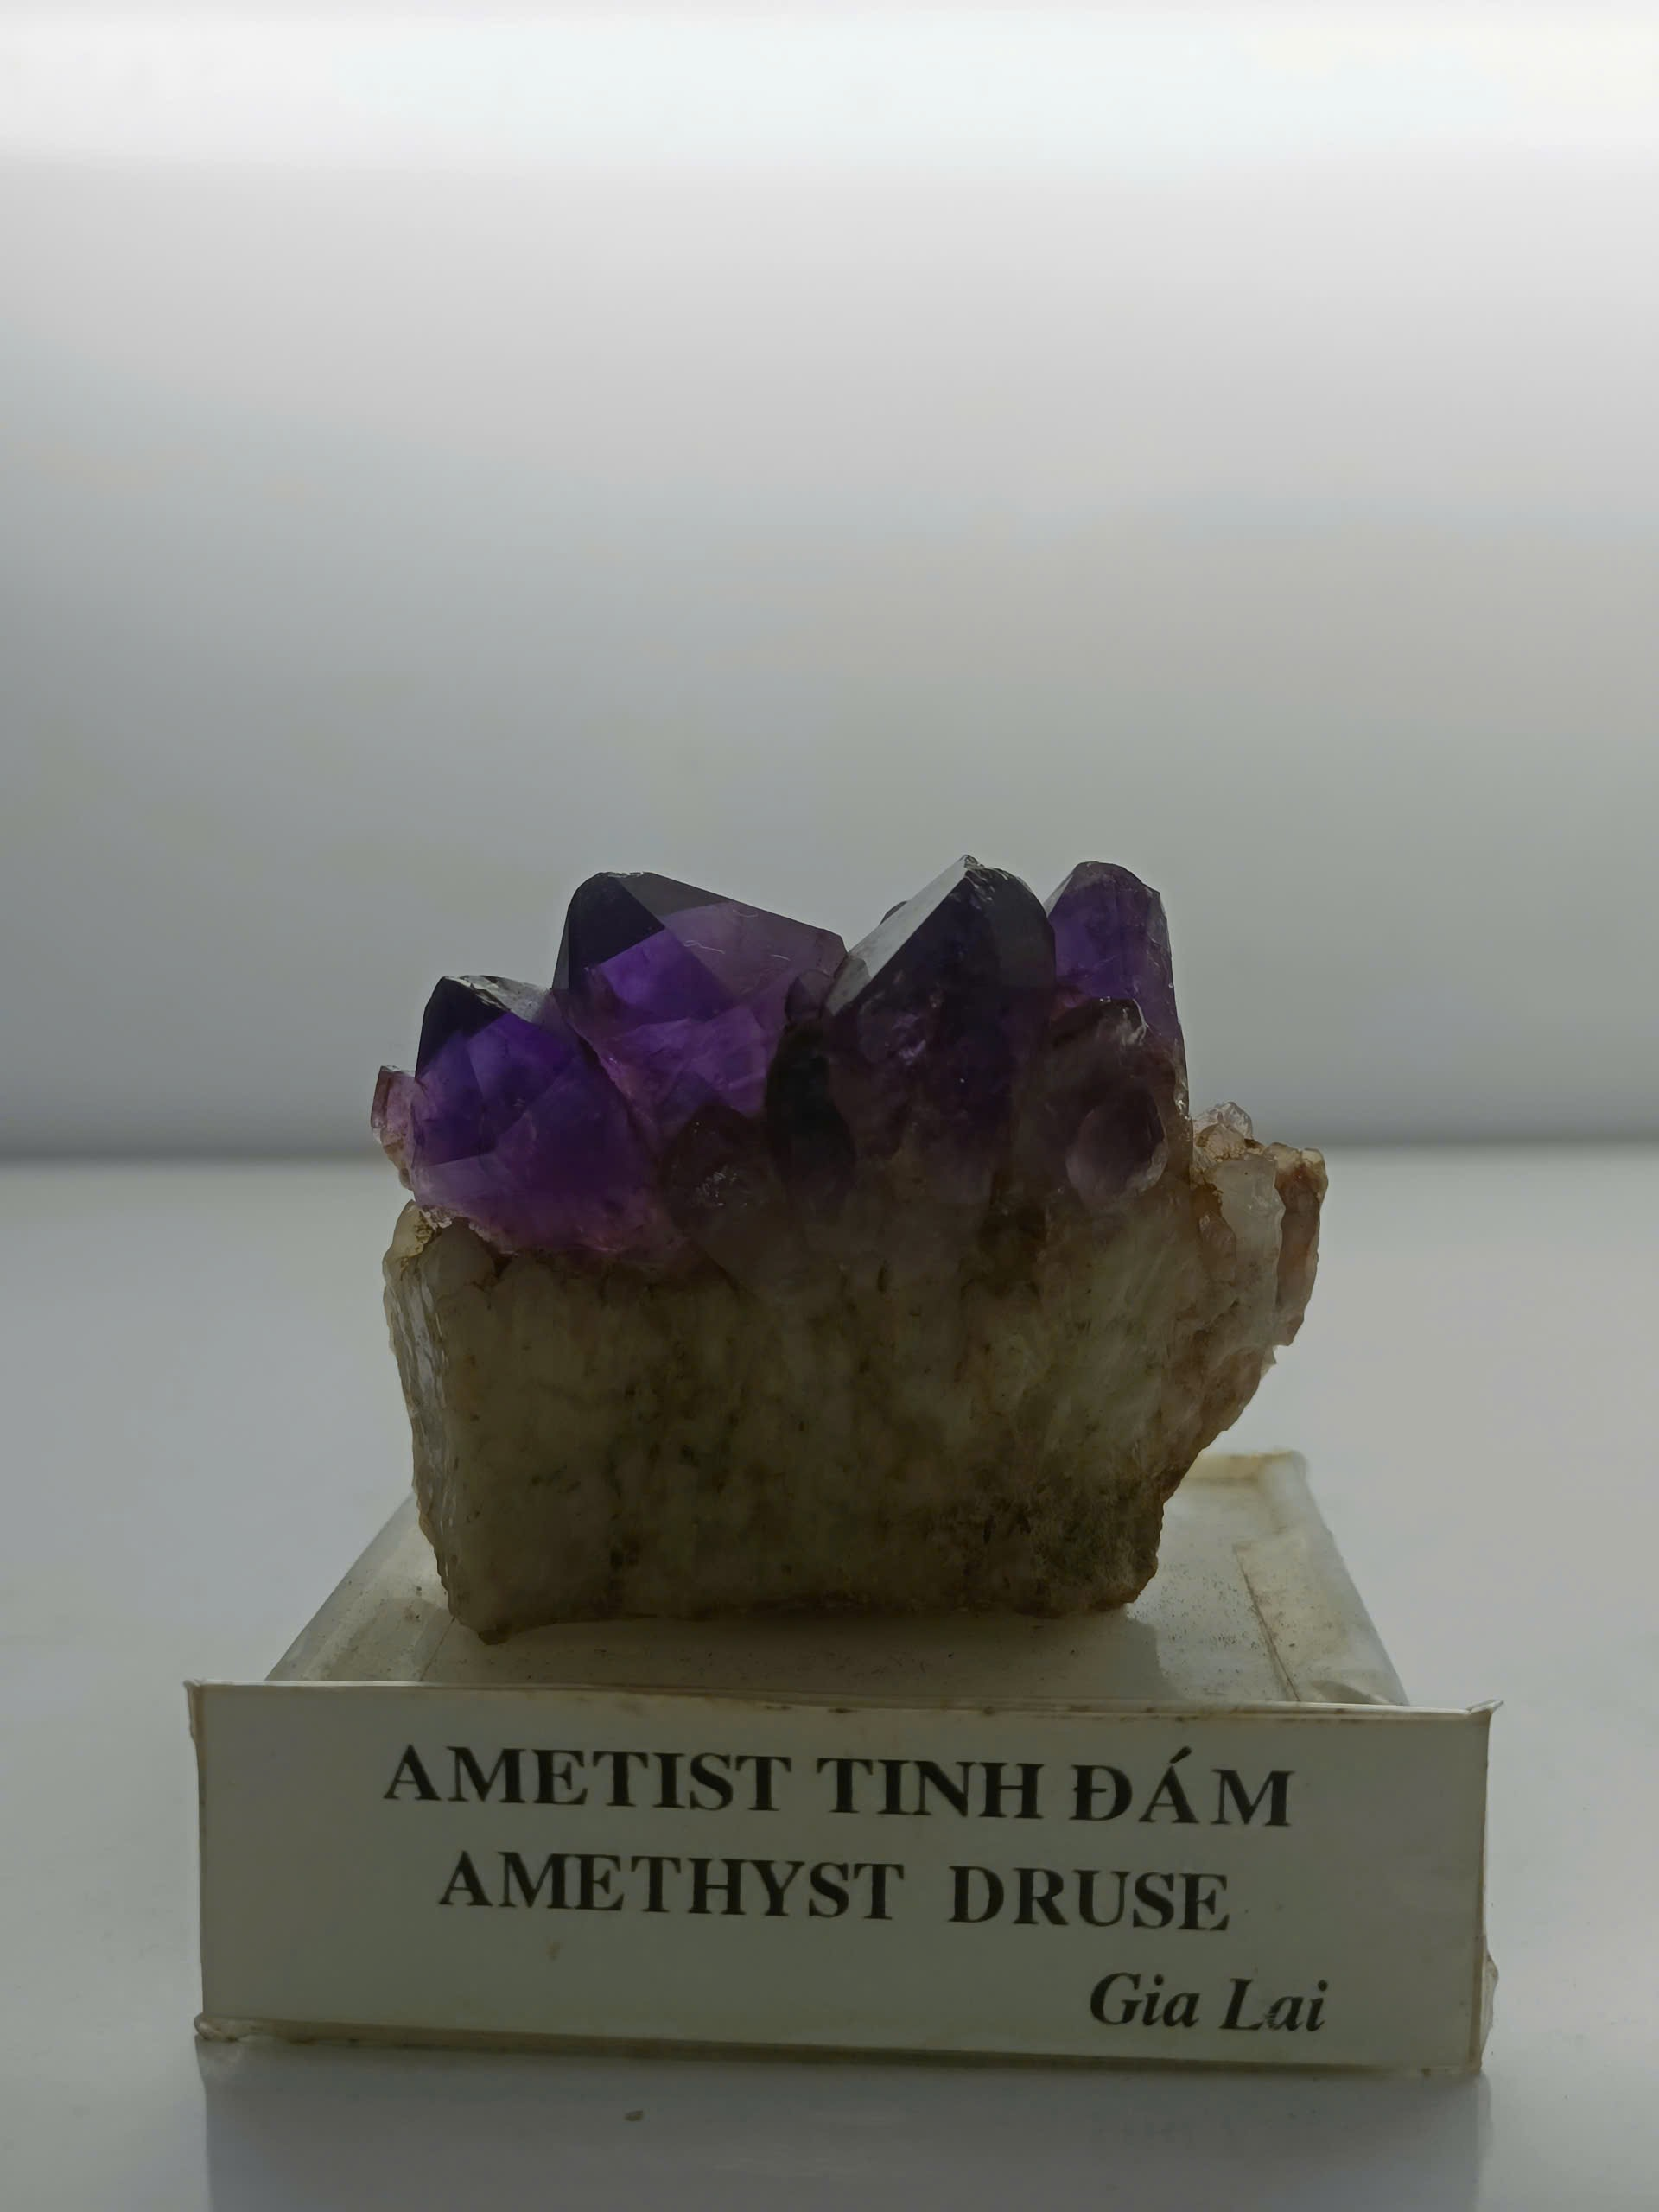
\includegraphics[width=0.7\textwidth]{graphics/amethyst.png}
\caption{Amethyst sample showing characteristic purple coloration}
\label{fig:amethyst}
\end{figure}

\textit{Chalcedony:} A cryptocrystalline form of silica composed of tiny quartz crystals. It typically has a waxy or glassy luster and comes in various colors including white, gray, blue, and brown. Chalcedony is commonly used in jewelry and decorative objects.



\textit{Quartz Crystals:} Clear crystalline quartz formations that are hexagonal in shape with pyramid-shaped termination points. These are used in both jewelry and industrial applications.

\begin{figure}[H]
\centering
\includegraphics[width=0.7\textwidth]{graphics/quartz_crystals.png}
\caption{Clear quartz crystals displaying hexagonal structure}
\label{fig:quartz_crystals}
\end{figure}

\textbf{Precious Gemstones}
\textit{Ruby:} A red variety of the mineral corundum, colored by trace amounts of chromium. Ruby is one of the most valuable gemstones and is highly prized for jewelry. Vietnamese rubies are found in marble formations and are known for their quality.

\begin{figure}[H]
\centering
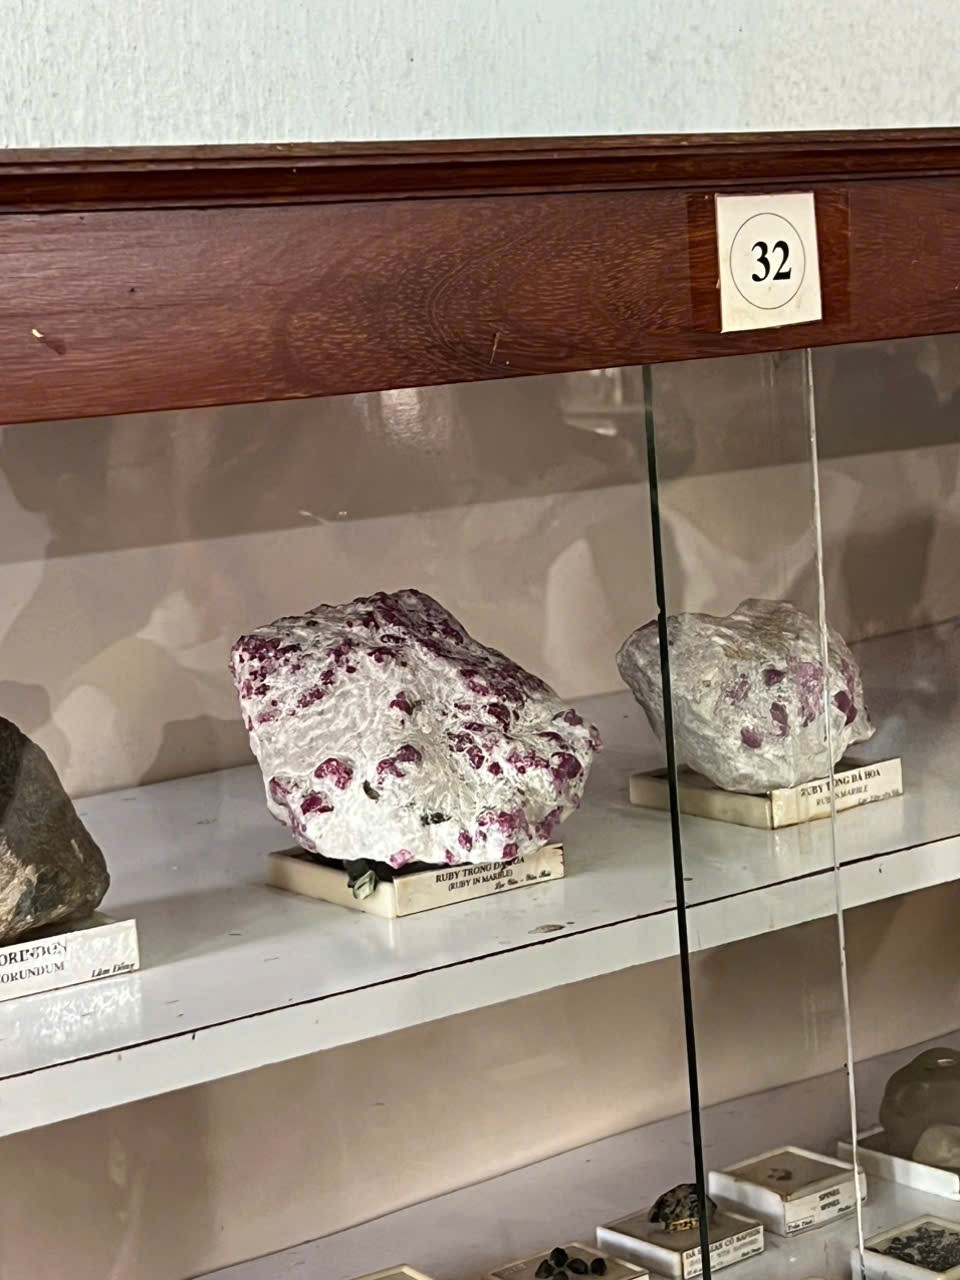
\includegraphics[width=0.7\textwidth]{graphics/ruby.png}
\caption{Ruby samples including ruby in marble matrix}
\label{fig:ruby}
\end{figure}

\textit{Topaz:} A rare silicate mineral with the chemical composition Al₂SiO₄(F,OH)₂. While pure topaz is colorless, trace elements can create various colors including blue, golden-brown, and yellow-orange. Topaz is valued for its hardness and brilliance in jewelry applications.

\begin{figure}[H]
\centering
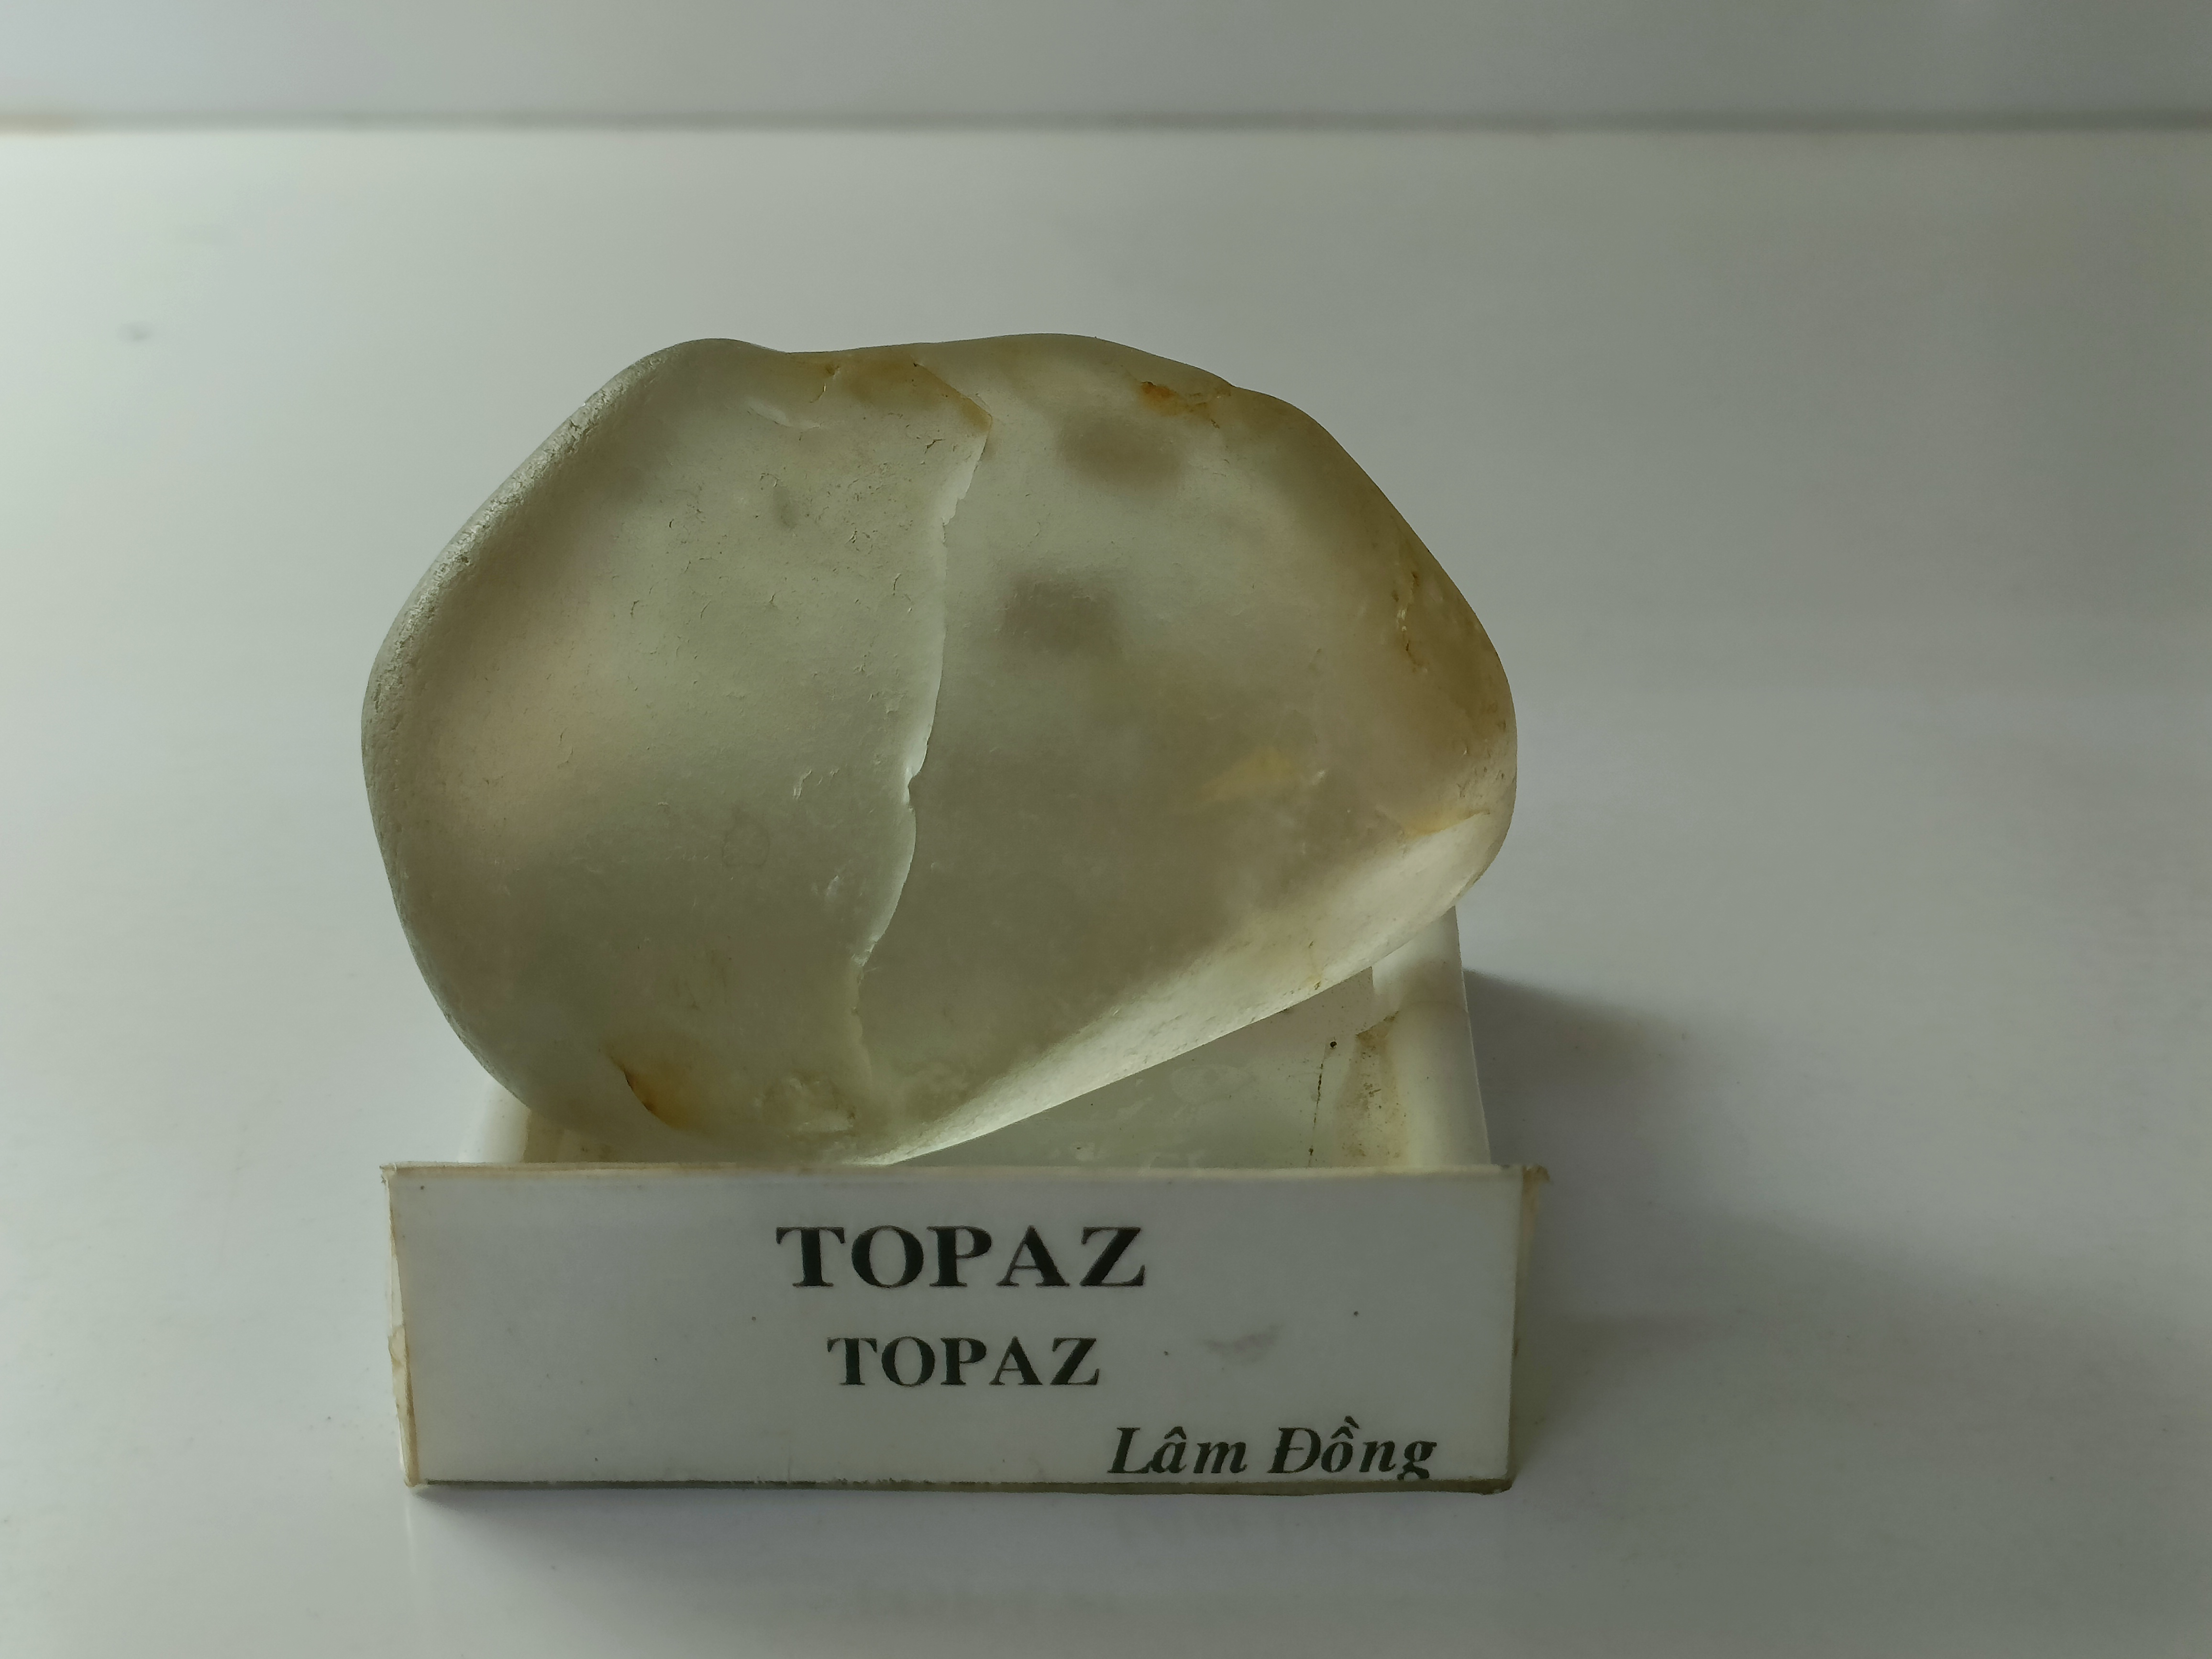
\includegraphics[width=0.7\textwidth]{graphics/topaz.png}
\caption{Topaz sample showing characteristic crystal structure}
\label{fig:topaz}
\end{figure}

\subsection{Mineral Water Resources}

Vietnam possesses significant mineral water resources with therapeutic and commercial value.

Natural mineral water is derived from underground sources where water has gradually acquired minerals while flowing through layers of rock over extended periods. Vietnam has numerous mineral water sources with diverse chemical compositions and therapeutic properties.

\textbf{Formation Process}
Groundwater penetrates deep underground, acquiring precious minerals and sometimes heating up in areas with tectonic activity, such as fault lines or historic volcanic zones. This process produces mineral-rich or hot springs that are geologically remarkable and recognized for their health benefits.

\textbf{Vietnamese Sources}
Vietnam has mineral water sources in various regions including Binh Thuan and Ninh Thuan provinces. Notable sources include:
\begin{itemize}
\item \textit{Vinh Hao:} Discovered by the French in 1928 in Vinh Hao, Tuy Phong, Binh Thuan
\item \textit{Van Lam:} Located in the northern regions
\item \textit{Ham Cuong:} Found in central Vietnam
\item \textit{Da Kai:} Another significant source
\end{itemize}

\textbf{Chemical Composition}
Vinh Hao mineral water, due to the perfect geological conditions of the Southeast Truong Son region with numerous interwoven rock layers, has:
\begin{itemize}
\item High concentration of bicarbonate (HCO$_3^-$) - acts as an antacid to reduce stomach acidity
\item Silicate dissolved in water - beneficial for digestion and nervous system
\item Calcium - prevents osteoporosis
\item Magnesium - strengthens immunity, improves heart function, and regulates blood pressure
\end{itemize}

\begin{figure}[H]
\centering
\includegraphics[width=0.7\textwidth]{graphics/mineral_water.png}
\caption{Mineral water samples from various Vietnamese sources}
\label{fig:mineral_water}
\end{figure}

\subsection{Geological Heritage}

Geological heritage represents a collection of geological resources with exceptional scientific, educational, artistic, and economic significance.

\textbf{Definition and Components}
Geological heritage refers to specific locations or landscapes on Earth that preserve evidence of the planet's formation and evolution, as well as the evolutionary history of life. Components include:
\begin{itemize}
\item Geomorphological landscapes
\item Paleontological sites and fossils
\item Extinct or active volcanic craters
\item Caves and river canyons
\item Natural lakes and waterfalls
\item Rock and ore exposures
\item Geological formations recording special events
\item Sites where geological processes can be observed
\end{itemize}

\textbf{Importance and Conservation}
Geological heritage sites have significant scientific, aesthetic, and historical importance, as well as tourism potential. Like other types of heritage, geological heritage is a finite resource that must be maintained, developed, and used sustainably.

\textbf{Vietnamese Context}
Vietnam's geological heritage includes diverse formations representing different geological periods and processes, from ancient Precambrian rocks to recent volcanic activity, providing valuable insights into Earth's history and geological evolution.
\section{Conclusion and Reflections}
\label{sec:conclusion}

\subsection{Summary of Key Findings}
\label{sec:summary_of_key_findings}
This report has documented our journey through the Ho Chi Minh City Geological Museum, providing a comprehensive overview of Vietnam's geological evolution and its rich mineral resources. We have explored the nation's geological history, from the ancient Precambrian formations to the dynamic processes of the Cenozoic era. The report detailed the formation of critical geological structures and examined the distribution of valuable mineral resources, including industrial metals, non-metallic minerals, and precious gemstones.

\subsection{Knowledge Gained}
\label{sec:knowledge_gained}
The process of researching and compiling this report has been an invaluable learning experience. It has provided us with a profound understanding of the geological forces that have shaped Vietnam's landscape and created its mineral wealth. This knowledge extends beyond theoretical concepts, offering practical insights that are crucial for the sustainable management and appreciation of our country's natural resources. As President Ho Chi Minh taught, "Learning must go hand in hand with practice," and this project has allowed us to bridge that gap.

\subsection{Vietnam's Mineral Resources and Geological Heritage}
\label{sec:vietnams_mineral_resources_heritage}
Vietnam's diverse mineral resources are a cornerstone of the national economy. This report has highlighted the significance of key minerals, from strategic metals to industrial materials and gemstones. However, their value is not purely economic. The geological formations that house these resources are a vital part of our natural heritage. Their preservation is essential for scientific research, education, and fostering a deeper connection with our environment. We believe that responsible resource management must be integrated with the conservation of this geological legacy.

\subsection{Personal Reflections}
\label{sec:personal_reflections}
This project has been more than an academic exercise; it has been a journey of discovery. Visiting the museum and studying the specimens firsthand brought the abstract concepts of geology to life. It has fostered a deep appreciation for the immense timescale of geological processes and the intricate beauty of the natural world. This experience has reinforced our understanding that geology is not just the study of rocks, but a way of understanding our planet's past, present, and future, and our responsibility to protect it.

\subsection{Acknowledgments}
\label{sec:acknowledgments}
We would like to express our sincere gratitude to our instructors and the staff at the Ho Chi Minh City Geological Museum. Your guidance, knowledge, and the stories you shared have been invaluable. This report is a testament to the knowledge we have gained, and we hope it reflects our best efforts to apply what we have learned. We also thank our team members for their collaboration and dedication in completing this project.

% Bibliography
\begin{thebibliography}{9}
\bibitem{thanhnien2023}
Thanh Niên. (2023). \textit{Bảo tàng ở TP.HCM: Bảo tàng Địa chất - Độc vị trái đất}. 
\url{https://thanhnien.vn/bao-tang-o-tphcm-bao-tang-dia-chat-doc-vi-trai-dat-18525040712390276.htm}
\end{thebibliography}

\end{document}
